\chapter{Interpreting Black-box Models}\label{chapter:xai}

\textit{"Predicting the future isn't magic, it's artificial intelligence."} -- Dave Waters 

\section{Chapter Overview}
In chapter \ref{chapter:uni_modality} and \ref{chapter:multiodality}, different modalities were considered to develop decision support system~(DSS) to leverage cancer types and subtypes prediction tasks. In both cases, the predictive models developed are mostly black-box methods. However, not only accurate diagnosis ~(i.e., predicting cancer types), but also revealing and interpreting biological significance about driver genes are vital for subsequent treatment. 

Besides, since data subjects are entitled to obtain meaningful information about logic, significance, and envisaged impacts of automated decision making, it is important to improve algorithmic transparency of the model based on which a DSS will be built upon. To improve the algorithmic transparency and explainability of the black-box models, different probing and interpretable methods are applied. Further, we validated our findings through functional analysis to make sure biomarkers are biologically trustworthy

\section{Introduction}\label{chapter_5:intro}
As the importance of genetic knowledge in cancer treatment is increasingly addressed, several projects have emerged, of which TCGA most well-known for omics data. Omics data is a collection of biomolecules inside living things such as genomics, metabolomics, and proteomics. TCGA curates various omics data, e.g., mutations, GE, DNA methylation, CNV, and miRNA expressions. By acquiring deep insights of these data, treatment can be focused on preventive measures. Besides, clinical and pathology information are provided. TCGA further analyzed over 11,000 cancer cases from 33 prevalent forms of cancer, which fostered the accomplishment of the Pan Cancer Atlas~(PCAt) project, covering gene expression, somatic mutation, DNA methylation, miRNA expression, and CNV~\cite{lyu2018deep}. 

\hspace*{3.5mm} In this chapter, multimodal genomics data is used to train deep neural network~(DNN) architectures to classify the cohorts into specific cancer patient groups. In particular, data from PCAt project~\cite{weinstein2013cancer} is used to train deep neural network~(DNN) architectures to classify the cohorts into specific cancer patient groups. In particular, a vanilla convolutional neural network~(CNN) and deep CNN architecture called VGG-16 are trained end-to-end for the classification. On the other hand, multimodal autoencoder~(MAE) and multimodal convolutional autoencoder~(MCAE) networks are to trained to learn joint latent representation from the multimodal genomics data before the classification.  
Diagnoses provided by the DSS consist of three steps: i) classifying cohort(s)~(group and individual) into specific cancer types based on their respective profiles, and ii) interpreting the prediction by highlighting biologically relevant biomarkers, and iii) explaining necessary logic involved in the diagnosis. These steps are based on two different strategies: based on single modality~(i.e., using single genomics data) and based on multimodality. %~(i.e., using different genomics data). 

\hspace*{3.5mm} To improve algorithmic transparency, different probing techniques are employed to open the `black-box' models. Since genomics data are high dimensional, we hypothesize\footnote{\textbf{H4}: \textit{Since genomics data is high dimensional, embedding them into 2D raw images can help locate significant~(i.e, most and least) biomarkers.}} that embedding them into 2D raw images can help locate significant~(i.e, most and least) biomarkers
\footnote{Supporting publication: \textbf{Md. Rezaul Karim}, Michael Cochez, Oya Beyan, Stefan Decker, and Christoph Lange-Bever, ``OncoNetExplainer: Explainable Predictions of Cancer Types Based on Gene Expression Data", Proc. of \emph{IEEE International Conference on Bioinformatics and Bioengineering~(BIBE'2019)}, Athens, Greece, October 28-30, 2019}. % for the corresponding tumor types. 
To identify relevant biomarkers\footnote{RQ2: \textit{How to identify relevant features or factors for a certain decision?}}, GradCAM++, attention mechanism, and LRP are used to generate class-specific heat maps~(HM) for all classes. 
Marker genes w.r.t prominent pixels position on 2D feature space are then marked, followed by computing their  importance in terms of mean absolute impact~(MAI). Top-k genes across cancer types are also ranked w.r.t MAI, followed by their functional analyses.  

%\footnote{Algorithmic transparency, w.r.t, post-model explainability.}. 
%Further, we validated our findings through functional analysis to make sure biomarkers are biologically trustworthy

\hspace*{3.5mm} The rest of the chapter is structured as follows: \cref{chapter_5:rw} covers related works concerning interpretable ML approaches and summarize their potential limitations. \Cref{chapter_5:mm} describes the overall approach, including the detail of the data collection and feature engineering before the network construction and training. \Cref{chapter_5:results} demonstrates the experiment results and discusses key findings of the study. \Cref{chapter_5:conclusion} provides explanations of the importance and relevance of the study reported, highlights the limitations and discuss future works before concluding the chapter.

\section{Related Work}\label{chapter_5:rw}
Lyu et al.~\cite{lyu2018deep} and Mostavi et al.~\cite{mostavi2019convolutional} embedded the RNA-Seq data from the PCA project into 2D images and trained a CNN to classify 33 tumor types, which outperforms the approach in~\cite{li2017comprehensive}. Besides, they provide a functional analysis of genes with high intensities in the HM based on Grad-CAM and validated that these top genes are related to tumor-specific pathways. Other general methods on explainability, fairness and robustness. 
%There is no prior art that handles a diverse set of desirable properties needed to develop a responsible AI system. 
Several other works introduced counterfactual explanations. However, their optimization formulation cannot handle categorical data~\cite{ying2019gnnexplainer}, i.e, optimization does not solve for such data and the values are found in a brute-force fashion.

\hspace*{3.5mm} \Cref{tab:multimodal_xai_approaches} and \cref{tab:global_vs_lical_xai} show the summarized views of the methods focusing interpretability, explainability, and transparency. Some other explainable methods works only for the linear models. Other approaches use a genetic algorithm to generate neighbors around the input and then use decision trees to locally approximate the model. However, local approximations might be at the cost of model accuracy, and they define counterfactual based on the minimum number of splits in the trained decision tree, which might not always be the smallest change to the input~\cite{li2017comprehensive}. They work on a white-box and simpler convolution models, and the distance metrics might not be apt to measure image similarity. 

\begin{table}[h]
    \centering
    \caption{XAI approaches w.r.t algorithmic fairness, robustness, and explainability on agnosticism}
    \label{tab:multimodal_xai_approaches}
    \scriptsize
    \vspace{-2mm}
    \begin{tabular}{l|l|l|l|l|l|l} 
        \hline
        \textbf{Reference}                & \textbf{Multimodality support} & \textbf{Black-box} & \textbf{Agnostic} & \textbf{Explainability} & \textbf{Fairness} & \textbf{Robustness}  \\ 
        \hline
        Shubham S. et al. 2019   & Yes                   & Yes       & Yes            & Yes            & Yes      & Yes         \\ 
        \hline
        Wacherer et al. 2019     & Yes                   & Yes       & No             & Yes            & Yes      & No          \\ 
        \hline
        Ustun et al. 2019        & No                    & Yes       & Yes            & Yes            & Yes      & No          \\ 
        \hline
        Russel et al. 2019       & Yes                   & Yes       & No             & Yes            & Yes      & No          \\ 
        \hline
        Ribeiro et al. 2016      & Yes                   & Yes       & Yes            & Yes            & No       & No          \\ 
        \hline
        Guidtit et al. 2016      & Yes                   & Yes       & Yes            & Yes            & No       & No          \\ 
        \hline
        Carlini \& Wagner, 2017 & No                    & No        & Yes            & No             & No       & Yes         \\ 
        \hline
        Weng et a. 2018          & No                    & No        & Yes            & No             & No       & Yes         \\ 
        \hline
        Karim et al. 2019        & No                    & Yes       & Yes            & Yes            & Yes      & No          \\
        \hline
    \end{tabular}
    \vspace{-4mm}
\end{table}

\hspace*{3.5mm} A few other approaches define a robustness score that need to have access to the model gradients. GNNExplainer is a recent approach for explaining the predictions by a graph neural network~(GNN)~\cite{ying2019gnnexplainer}. Given a trained GNN model and an input instance, GNNExplainer can generate the explanations via a dense subgraph. Secondly, GNNExplainer can be applied across tasks, e.g., node classification, graph classification, and link prediction, in a task-agnostic way. Thirdly, GNNExplainer can be employed on different GNN models such as GCN, GraphSAGE, GAT, and SGC to generate corresponding explanations. 

\begin{table}[h]
    \centering
    \scriptsize
    \caption{Approaches to interpretability of ML models based on agnosticism}
    \label{tab:global_vs_lical_xai}
    \vspace{-2mm}
    \begin{tabular}{l|l|l} 
        \hline
        \textbf{Agnosticism}  & \textbf{Global interpretability}  & \textbf{Local interpretability} \\ 
        \hline
        \multirow{4}{*}{Model specific} & Regression (logistic/linear) models & Individual (e.g., patient) specific set of decision rules \\ 
        \cline{2-3}
        & Decision trees & Tree decomposition of decision rules \\ 
        \cline{2-3}
        & Naïve Bayes & K-nearest neighbour (KNN)\\ 
        \cline{2-3}
        & GNN Explainer~\cite{GNNEXPLAINER} & GNN Explainer~\cite{GNNEXPLAINER} \\ 
        \hline
        \multirow{5}{*}{Model agnostic} & Global surrogate models  & Local interpretable model-agnostic explanation (LIME)~\cite{LIME}\\ 
        \cline{2-3}
        &  MUSE  & Shapely additive explanations (SHAP)~\cite{SHAP}\\ 
        \cline{2-3}
        & Partial dependence plots (PDP) & Anchors~\cite{ribeiro2018anchors} \\ 
        \cline{2-3}
        & Summary plot showing global feature importance & MUSE \\ 
        \cline{2-3}
        & BETA~\cite{BETA} & Sailency and attention maps (e.g., CAM)\\ 
        \hline
    \end{tabular}
    \vspace{-4mm}
\end{table}

\hspace*{3.5mm} Due to the stochastic nature of DNN, the prediction and feature importance generated would be slightly different across runs, i.e., not deterministic. This also applied to DSS we developed in the previous chapters. We might even encounter similar issue for tree-based ensemble models such as random forest. For example, GBT provides 3 options for measuring feature importance: i) \emph{weight}, which is the number of times a feature is used to split the data across all trees, ii) \emph{cover}, the number of times a feature is used to split the data across all trees weighted by the number of training data points go through those splits, and iii) \emph{gain}, which is the average training loss reduction gained when using a feature for splitting. Based on these measure, feature importance orderings~(i.e., the order in which features were added) are different since subsequent features will get a disproportionately high weight.

\section{Methods}\label{chapter_5:mm}
In this section, we discuss our approach in detail, including data collection, preprocessing, network construction, and training, followed by interpreting the network towards biomarkers identification. There is no single approach to explainable AI that always works best~\cite{arya2019one}. There are many ways to explain an algorithmic decision or a model. The appropriate choice depends on the persona of the consumer and the requirements of the AI pipeline that bridge the gap from research to practice~\cite{arya2019one}. Based on this insights, we rely on several probing and interpretability methods discussed in \cref{chapter:preli}

\subsection{Problem statement}
From given genomics profiles of PCAt cohorts consisting of GE, DNA methylation, and miRNA expressions, the problem is to classify the patients into specific cancer types. Given $n$ samples, $X$ = ${{\{x_1,x_2, ..., x_n}}\}$ in dataset $D$, where $X \in {R}^{D}$. We consider classifying an individual $x$ into a specific cancer type based on its respective profiles, but in two different ways: i) based on single modality, ii) based on multimodality, where a  classifier is a function $f: {X}^{(m)} \rightarrow {Y}$, which maps a data instance $x$ from a feature space ${X}^{(m)}$ with $m$ input features to a labels $y$ in a target space ${Y}$, where $f(x)=y$ denotes the decision $y$ predicted by $f$, and input instance $x$ consists of a set of $m$ attribute-value pairs $\left(a_{i}, v_{i}\right)$ in which $a_i$ is a feature and $v_i$ is a value from the domain of $a_i$. 

\hspace*{3.5mm} In \cref{chapter:uni_modality}, we developed two `black-box' predictors: let's say $F$ is the first predictor whose internal functioning is either unknown to the observer or they are known but not interpretable by a human. In this chapter, we assume $F$ lacks of explainability by default, in which we embed local and global explainability logic to make it interpretable, which we hope to explain a data point $x$ using an explanation function $g$. We denote ${F}$ - an interpretable predictor, whose internal processing yielding a decision ${F}(x)=y$ can be given a symbolic interpretation understandable by a human. 

\hspace*{3.5mm} While using single modality, we classify samples directly in it's original data space $X$. In the latter approach, instead of classifying samples directly in it's original data space $X$, we first transform each data with a nonlinear mapping $f_{\theta}: X \rightarrow Z$, where $\theta$ are learnable parameters and $Z \in {R}^{K}$ is the learned or embedded feature space, where $K \ll D$. Then we create a shared representation of class-discriminating features from each modality, followed by parametrizing $f_{\theta}$ by representation learning based on multimodal convolutional autoencoders~(MCAE) is employed due to it's function approximation properties and feature learning capabilities~\cite{xie2016unsupervised,karim2019drug} from genomic data. Based on embedding $Z$, the classifier then $f$ maps an input $x$ to an output $f(x) \in y, f: {R}^{d} \mapsto y$. When we assume $f$ has a parametric form, we write $f_{\theta}$, where ${L}(f(x), y)$ denotes the loss function used to train $f$ on a dataset $D$ of input-output pairs $(x(i), y(i))$. Local explainability refers to an explanation for why $f$ predicted $f(x)$ for a fixed point $x$. 
%The local explanation methods we discuss come in one of the following forms: which feature $x_i$ of $x$ was most important for prediction with $f$? Which training data point $Z \in \mathbb{R}^{K}$ was most important to $f(x)$? What is the minimal change to the input $x$ required to change the output $f(x)$? 

\subsection{Datasets}
The DNA methylation, copy numbers, mutations, miRNA, and GE profiles from PCAt covering 33 prevalent tumor type for 9,074 samples are considered in our approach. This dataset has been used widely as prior knowledge to generate tumor-specific biomarkers~\cite{way2018machine,hoadley2018cell,malta2018machine}. These data are hybridized by the Affymetrix Genome-Wide Human SNP Array 6.0\footnote{\url{http://www.affymetrix.com/support/technical/byproduct.affx}}, which allows us to examine the largest number of cases along with the highest probe density~\cite{31Park}. Besides, we use the cancer transcriptomes from the PCAt project to interrogate GE states induced by deleterious mutations and copy number alterations. The sample distribution across data types are shown in \cref{table:alldatadetails2}~\cite{weinstein2013cancer}. 

\begin{table} [h]
\centering
    \scriptsize
    \caption{Sample distribution across tumor types: rows: tumour type, column: data types~\cite{weinstein2013cancer}}
    \label{table:alldatadetails2}
    %\vspace{-2mm}
    \begin{tabular}{l|l|l|l|l|l|l}
        \hline
        \rowcolor{Gray}
         \textbf{Cohort} & \textbf{DNA meth.} & \textbf{Copy numbers} & \textbf{Mutations} & \textbf{miRNA} & \textbf{Gene expr.} & \textbf{Carcinoma type} \\\hline
            LUSC & 358 & 345 & 178 & 332 & 227 & Lung squamous cell carcinoma \\\hline
            READ & 162 & 164 & 69 & 143 & 71 & Rectum adeno-carcinoma \\%
            GBM  & 405 & 578 & 290 & 501 & 495 & Glioblastoma multiforme \\\hline
            LAML & 194 & 198 & 197 & 187 & 179 & Acute myeloid leukemia	\\%
            HNSC & 310 & 310 & 277 & 309 & 303 & Head \& neck squamous cell carcinoma \\\hline 
            BLCA & 126 & 126 & 99 & 121 & 96 & Bladder urothelial carcinoma \\\hline 
            KIRC & 457 & 457 & 417 & 442 & 431 & Kidney renal clear cell carcinoma  \\\hline
            UCEC & 512 & 511 & 248 & 497 & 333 & Uterine corpus endometrial carcinoma \\\hline
            LUAD & 431 & 357 & 229 & 365 & 355 & Lung adenocarcinoma \\\hline
            OV   & 592 & 577 & 316 & 454 & 581 & Ovarian serous cystadenocarcinoma \\\hline
            BRCA & 888 & 887 & 772 & 870 & 817 & Breast invasive carcinoma  \\\hline
            COAD & 420 & 422 & 155 & 407 & 192 & Colon cdenocarcinoma \\\hline
            %LGG  & 514 & 487 & Brain lower grade glioma \\\hline
            %THCA & 505 & 513 & Thyroid carcinoma \\\hline 
            %PRAD & 501 & 536 & Prostate adenocarcinoma \\\hline 
            %STAD & 442 & 464 & Stomach adenocarcinoma \\\hline 
    \end{tabular}
    \vspace{-2mm}
\end{table}

\subsection{Feature selection}
One of the goals of genomics data~(in particular, expression data) analysis is to disseminate biologically meaningful information about the biomarkers such as genes and proteins. 
%Through these information, biologists are able to discover unknowns and reaffirm previously knowledge. 
Since, our aims is providing accurate diagnosis of cancer, information about gene interaction is of biological relevance. This will provide clearer understanding of the roles a certain set of genes play in cancer development and related issues, which will also assists in the  early treatment of disease~\cite{lu2003cancer}. %It is a common consensus that biological relevance for a cancer classifier is as important as the classification
%accuracy.

\hspace*{3.5mm} Identification of biomarkers is the ranking of biologically significant and meaningful features, which is based on individual feature correlation w.r.t class separation, i.e., selecting genes with high individual correlation with the classes such that no correlation among the genes Finding marker genes that are genes whose expression values are biologically useful for determining the class of the samples~\cite{lu2003cancer}. In other words, marker genes are genes that characterize the tumor classes. Subsequently, accurate identification of marker genes are important due to the following reasons~\cite{lu2003cancer}:

\begin{itemize}[noitemsep]
    \item Enable better classification performance
    \item Allow biologists further study the interaction of relevant genes 
    \item Study the functional and sequential behavior of known marker genes in order to facilitate the functionality discovery of other genes.
    \item Allow further study of relation of expression values of different genes with respect to the tumor class, is similar expression pattern always results in cancer or the combination of suppression of certain genes and expression of certain genes are a better indication of tumor, etc.
\end{itemize}

%It has also been observed that for the same gene selection mechanism, the accuracies of different classifiers do not differ much, whereas different gene selection methods have greater effect on the classification accuracy. This again proved how an important role gene selection plays in cancer classification. In conclusion, we feel that a good gene selection method for cancer classification should observe the
%following properties:
%corporation of the gene interaction information,
%- selection criteria based on group performance instead of individual correlation,
%. Inclusion of complementary genes, Picking of cancer related genes instead of cell composition related genes, and
%. Reasonably efficient.

\iffalse
\begin{table} [!ht] 
    \begin{center}
    \scriptsize
    \caption{gene expression sample distribution across tumor types}
        \vspace{-2mm}
    \label{table:GE_dist}
    \begin{tabular}{l|l|l}
        \toprule
        %\rowcolor{Gray}
         \textbf{Cohort} & \textbf{\#Sample} & \textbf{Carcinoma type} \\\midrule
         BRCA & 981  & Breast invasive carcinoma  \\%
         LGG  & 507  & Brain lower grade glioma \\% 
         UCEC & 507  & Uterine endometrial carcinoma \\%
         LUAD & 502  & Lung adeno-carcinoma \\%
         HNSC & 487  & Head-neck squamous cell carcinoma \\% 
         THCA & 480  & Thyroid carcinoma \\%
         PRAD & 479  & Prostate adeno-carcinoma \\%
         LUSC & 464  & Lung squamous cell carcinoma \\%
         BLCA & 398  & Bladder urothelial carcinoma \\%
         STAD & 383  & Stomach adeno-carcinoma \\%
         SKCM & 363  & Skin cutaneous melanoma \\%
         KIRC & 352  & Kidney renal clear cellcarcinoma  \\%
         LIHC & 348  & Liver hepato-cellular carcinoma	\\%
         COAD & 341  & Colon adeno-carcinoma \\%
         CESC & 272  & Cervical \& endo-cervical cancer \\%
         KIRP & 271  & Kidney papillary cell carcinoma	\\%
         SARC & 229  & Sarcoma \\%
         OV   & 176  & Ovarian serouscystadenocarcinoma \\%
         ESCA & 169  & Esophageal carcinoma \\%
         PCPG & 161  & Pheochromocytoma-paraganglioma \\%
         PAAD & 152  & Pancreatic adenocarcinoma	\\%
         TGCT & 144  & Testicular germ cell tumor \\%
         GBM  & 124  & Glioblastoma multiforme \\%
         THYM & 119  & Thymoma	 \\%
         READ & 118  & Rectum adeno-carcinoma \\%
         LAML & 115  & Acute myeloid leukemia	\\%
         MESO & 82  & Mesothelioma	\\%
         UVM & 80  & Uveal melanoma	 \\%
         ACC & 76  & Adrenocortical cancer	\\%
         KICH & 65  & Kidney chromophobe	\\%
         UCS & 56  & Uterine carcino-sarcoma	 \\%
         DLBC & 37  & Diffuse large B-cell lymphoma	\\%
         CHOL & 36  & Cholangio carcinoma	 \\%
         \bottomrule
    \end{tabular}
    \end{center}
\end{table}
The distributions of miRNA of somatic mutations samples are shown in \cref{table:MIRNA_dist} and \cref{table:SM_dist}. 
\begin{table} [!ht] 
    \begin{center}
    \scriptsize
    \caption{miRNA expression sample distribution across tumor types}
        \vspace{-2mm}
    \label{table:MIRNA_dist}
    \begin{tabular}{l|l|l}
        \toprule
        %\rowcolor{Gray}
         \textbf{Cohort} & \textbf{\#Sample} & \textbf{Carcinoma type} \\\midrule
         BRCA & 981  & Breast invasive carcinoma  \\%
         LGG  & 507  & Brain lower grade glioma \\% 
         UCEC & 507  & Uterine endometrial carcinoma \\%
         LUAD & 502  & Lung adeno-carcinoma \\%
         HNSC & 487  & Head-neck squamous cell carcinoma \\% 
         THCA & 480  & Thyroid carcinoma \\%
         PRAD & 479  & Prostate adeno-carcinoma \\%
         LUSC & 464  & Lung squamous cell carcinoma \\%
         BLCA & 398  & Bladder urothelial carcinoma \\%
         STAD & 383  & Stomach adeno-carcinoma \\%
         SKCM & 363  & Skin cutaneous melanoma \\%
         KIRC & 352  & Kidney renal clear cellcarcinoma  \\%
         LIHC & 348  & Liver hepato-cellular carcinoma	\\%
         COAD & 341  & Colon adeno-carcinoma \\%
         CESC & 272  & Cervical \& endo-cervical cancer \\%
         KIRP & 271  & Kidney papillary cell carcinoma	\\%
         SARC & 229  & Sarcoma \\%
         OV   & 176  & Ovarian serouscystadenocarcinoma \\%
         ESCA & 169  & Esophageal carcinoma \\%
         PCPG & 161  & Pheochromocytoma-paraganglioma \\%
         PAAD & 152  & Pancreatic adenocarcinoma	\\%
         TGCT & 144  & Testicular germ cell tumor \\%
         GBM  & 124  & Glioblastoma multiforme \\%
         THYM & 119  & Thymoma	 \\%
         READ & 118  & Rectum adeno-carcinoma \\%
         LAML & 115  & Acute myeloid leukemia	\\%
         MESO & 82  & Mesothelioma	\\%
         UVM & 80  & Uveal melanoma	 \\%
         ACC & 76  & Adrenocortical cancer	\\%
         KICH & 65  & Kidney chromophobe	\\%
         UCS & 56  & Uterine carcino-sarcoma	 \\%
         DLBC & 37  & Diffuse large B-cell lymphoma	\\%
         CHOL & 36  & Cholangio carcinoma	 \\%
         \bottomrule
    \end{tabular}
    \end{center}
\end{table}
\begin{table} [!ht] 
    \begin{center}
    \scriptsize
    \caption{somatic mutation sample distribution across tumor types}
        \vspace{-2mm}
    \label{table:SM_dist}
    \begin{tabular}{l|l|l}
        \toprule
        %\rowcolor{Gray}
         \textbf{Cohort} & \textbf{\#Sample} & \textbf{Carcinoma type} \\\midrule
         BRCA & 981  & Breast invasive carcinoma  \\%
         LGG  & 507  & Brain lower grade glioma \\% 
         UCEC & 507  & Uterine endometrial carcinoma \\%
         LUAD & 502  & Lung adeno-carcinoma \\%
         HNSC & 487  & Head-neck squamous cell carcinoma \\% 
         THCA & 480  & Thyroid carcinoma \\%
         PRAD & 479  & Prostate adeno-carcinoma \\%
         LUSC & 464  & Lung squamous cell carcinoma \\%
         BLCA & 398  & Bladder urothelial carcinoma \\%
         STAD & 383  & Stomach adeno-carcinoma \\%
         SKCM & 363  & Skin cutaneous melanoma \\%
         KIRC & 352  & Kidney renal clear cellcarcinoma  \\%
         LIHC & 348  & Liver hepato-cellular carcinoma	\\%
         COAD & 341  & Colon adeno-carcinoma \\%
         CESC & 272  & Cervical \& endo-cervical cancer \\%
         KIRP & 271  & Kidney papillary cell carcinoma	\\%
         SARC & 229  & Sarcoma \\%
         OV   & 176  & Ovarian serouscystadenocarcinoma \\%
         ESCA & 169  & Esophageal carcinoma \\%
         PCPG & 161  & Pheochromocytoma-paraganglioma \\%
         PAAD & 152  & Pancreatic adenocarcinoma	\\%
         TGCT & 144  & Testicular germ cell tumor \\%
         GBM  & 124  & Glioblastoma multiforme \\%
         THYM & 119  & Thymoma	 \\%
         READ & 118  & Rectum adeno-carcinoma \\%
         LAML & 115  & Acute myeloid leukemia	\\%
         MESO & 82  & Mesothelioma	\\%
         UVM & 80  & Uveal melanoma	 \\%
         ACC & 76  & Adrenocortical cancer	\\%
         KICH & 65  & Kidney chromophobe	\\%
         UCS & 56  & Uterine carcino-sarcoma	 \\%
         DLBC & 37  & Diffuse large B-cell lymphoma	\\%
         CHOL & 36  & Cholangio carcinoma	 \\%
         \bottomrule
    \end{tabular}
    \end{center}
\end{table}
\fi 
%\subsection{Network construction and training}
%\label{subsec:nc_tr}
%In this subsection, we discuss the data preparation, network construction, training, followed by interpreting the network towards biomarkers identification.   

\subsection{Unimodal CNN models}
In this subsection, we discuss construction and training of the unimodal vanilla CNN and VGG16 models. Then we cover the detail of interpreting these black-box models. To show the effectiveness, only GE profiles are used to train each CNN architecture. Workflow of the overall approach is shown in \cref{fig:workflow_2D_CNN}.

\begin{sidewaysfigure*}
	\centering
	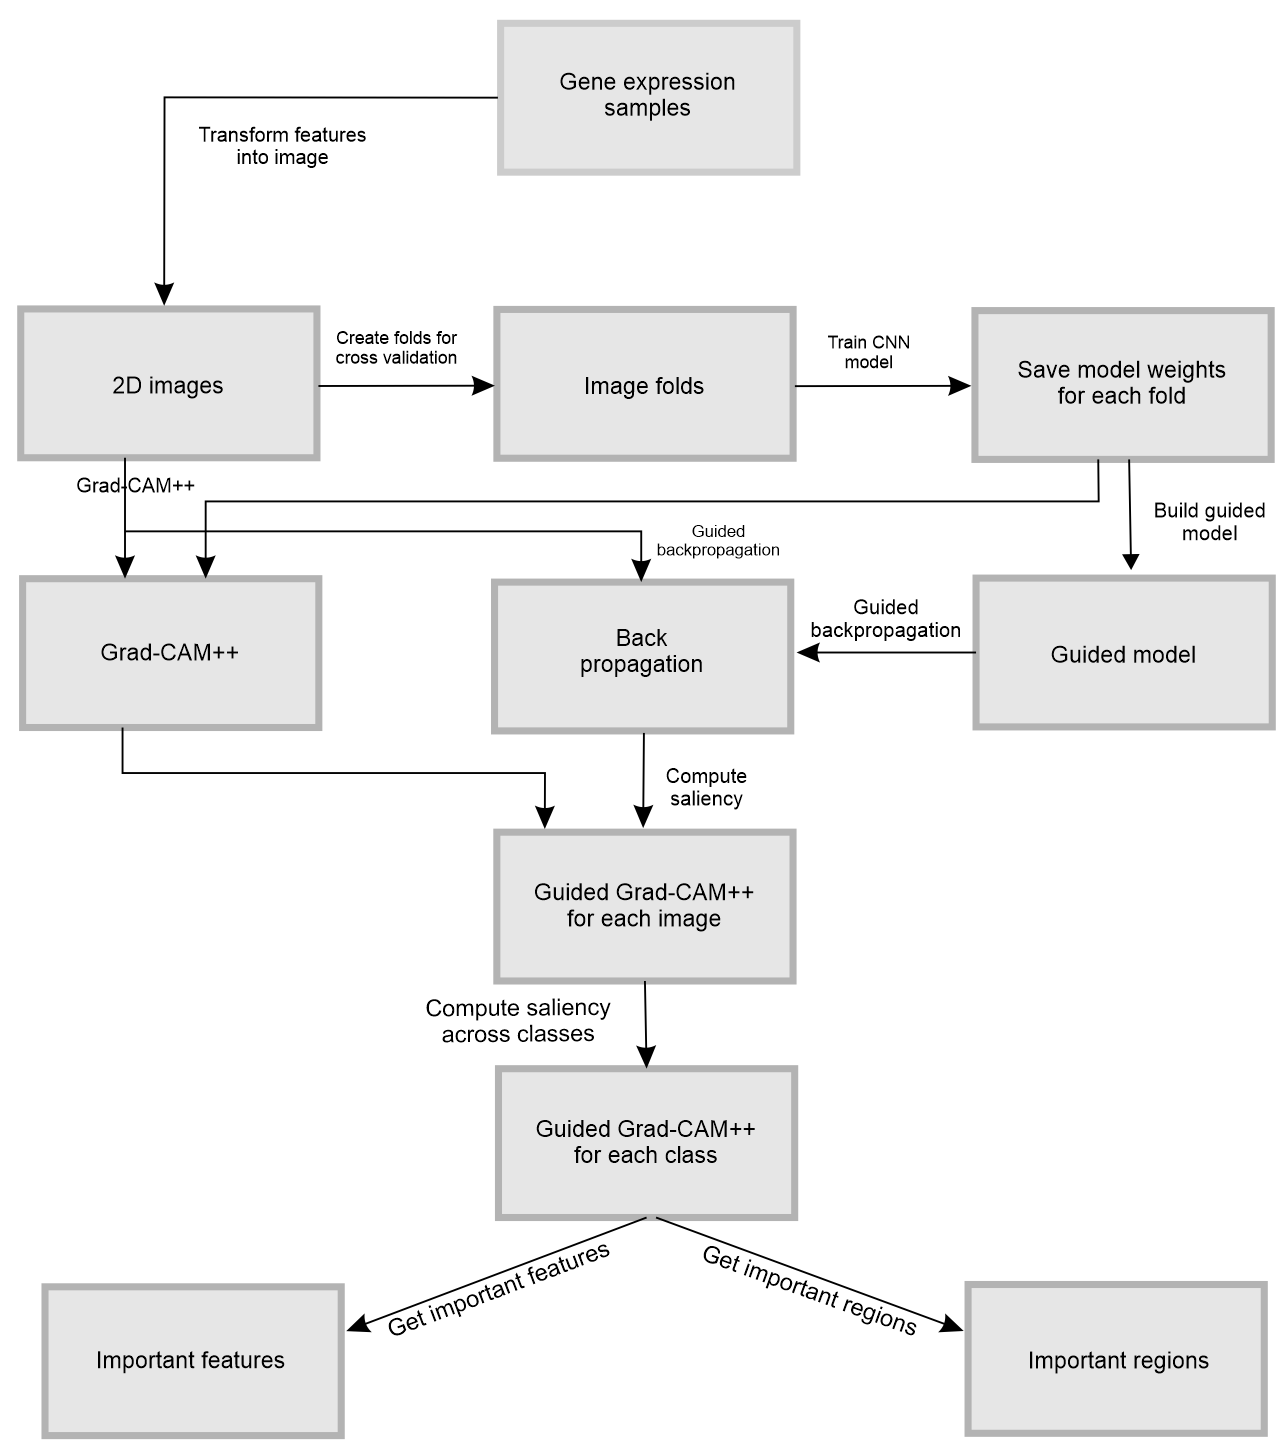
\includegraphics[scale=1.0]{images/wf_2D_CNN.png}
    \caption{Workflow of the unimodal CNN modality approach}	
	\label{fig:workflow_2D_CNN}
\end{sidewaysfigure*}

\subsubsection{Preprocessing}
Since we are interested in finding the relations between instances, e.g., GE of a particular cohort in relation to other types tumors, we use the the normalized version of the `GE RNA-seq' data. The expression values are generated at UCSC by first combining `GE RNA-seq' values higher than that of all TCGA cohorts and then mean normalizing all values per gene. The data is subsequently divided into the 30-40\% types to make the distribution balanced across cancer types and can serve as a proxy of background distribution of GE. To perform 2D  convolutional~(conv) operations, first we embed GE samples into 2D images in which GE values for each sample are reshaped from a 20,501$\times$1 array into a 144$\times$144 image by zero padding around the edges and normalized to [0,255].%, without losing any information.

\subsubsection{Network construction and training}
%However, prior applying the convolutional~(conv) operations, similar to \cref{chapter:uni_modality}, we first embed the samples into 2D images in which respective features for each sample are transformed into gray-scale image by zero padding around the edges and normalized to [0,255]. All the images are then normalized to [0,255], without losing any information. 
Both vanilla CNN and VGG16 architectures are trained from scratch alongside data augmentation in which the output of each convolutional layer is passed to dropout and Gaussian noise layer to avoid overfitting and thus regularize the learning~\cite{vardropout}. This involves the input feature space into a lower-dimensional representation, which is then further down-sampled by two different pooling layers and a max-pooling layer~(MPL) by setting the pool size. The output of an MPL is considered as an `extracted feature' from each 2D GE image. Since each MPL `flattens' the output space by taking the highest value in a FM, this produces a sequence vector from the last convolutional layer, which we expect to force the GE value of specific genes that are highly indicative of being responsible for a specific cancer type. Then this vector is passed through another dropout, and then softmax layers for the probability distribution over the classes.

\begin{figure*}[h]
	\centering
	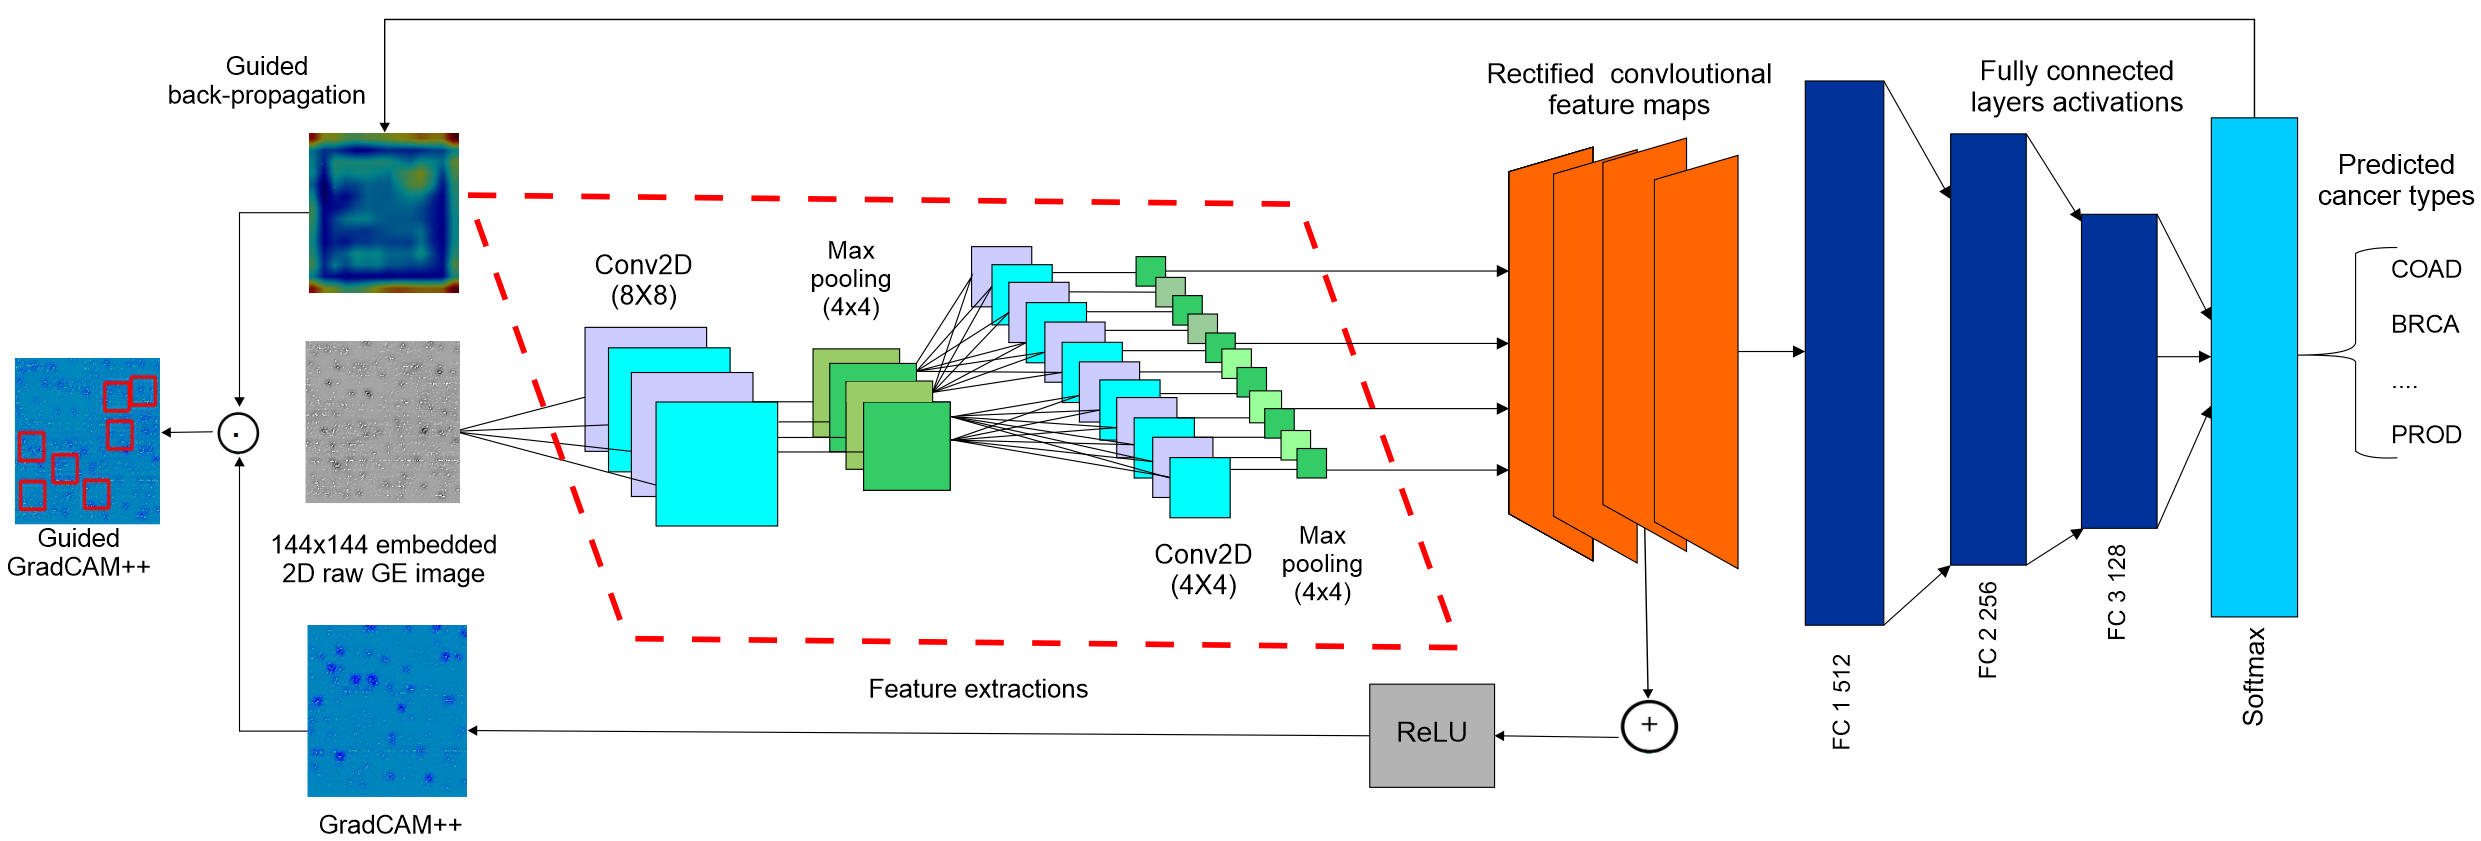
\includegraphics[scale=0.55]{images/clstm.PNG}
    \caption{Schematic representation of CNN-based approach, which starts by taking a raw GE sample as input and passing it through convolutional and pooling layers to generate rectified convolutional feature maps. Feature maps are then passed through fully connected softmax layer for classification. Guided back-propagation and Grad-CAM++ are applied to identify important important genes w.r.t pixel values.}	
	\label{fig:clstm}
\end{figure*}

\hspace*{3.5mm} Besides, VGG16 is also trained from scratch instead of initializing it's network weight from pretrained models. The reason is that, for example, ImageNet contains photos of general objects, which would activate the internal representation of network's hidden layers with geometrical forms, colorful patterns, or irrelevant shapes that are usually not present in biological datasets~\cite{Karim2020DeepCOVIDExplainer}. Both CNN architectures are trained with first-order gradient-based AdaGrad optimizer to optimize following categorical cross-entropy loss between predicted $Y^{\prime}$ and actual cancer type $Y$: 

\vspace{-2mm}
\begin{equation} 
    L_{ccae}=-\sum_{k=1}^{D}\left[Y_{k} \log Y_{k}^{\prime}+\left(1-Y_{k}\right) \log \left(1-Y_{k}^{\prime}\right)\right]
    \label{eq:cross_entropy_loss_2}
\end{equation} 

\hspace*{3.5mm} Softmax activation function is used in the output layer for the probability distribution over the classes for breast cancer subtype prediction. Further, we observe the performance by adding the Gaussian noise layer followed by the dense layer to improve model generalization and reduce overfitting, where the Gaussian noise parameters are empirically set to a standard deviation of 0.1 and a mean of 0. Since an appropriate selection of hyperparameters can have a huge impact on the performance of a deep architecture, we perform the hyperparameter optimization through random search and 5-fold cross-validation tests. 

\begin{figure*}[h]
	\centering
	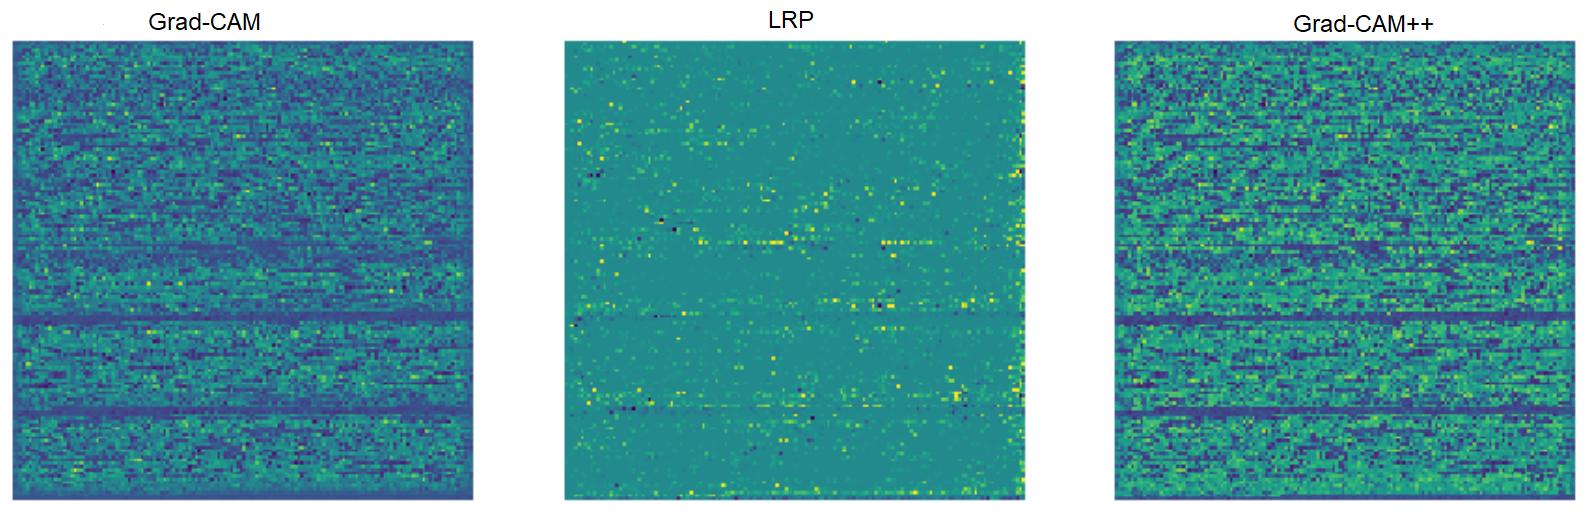
\includegraphics[scale=0.8]{images/3_mode.png}
	\caption{Heat map examples for a single cancer type prediction, where the image-pixel of specific biomarkers are highlighted by probing the network with Grad-CAM, Grad-CAM++, and LRP.} 
	\label{fig:3hms}
\end{figure*}

\subsubsection{Interpreting black-box CNN models}
Since the data is very high dimensional, we chose not to go for manual feature selection. Rather, we let both CNN and VGG16 networks extract the most important features. \Cref{algo:hm} and \ref{algo:imp_area} depict the pseudo-codes for computing feature importance with ranking genes and identification of important areas on the HM, respectively. We averaged all the normalized HM from the same class to generate a class-specific HM inspired by Selvaraju et al.~\cite{mostavi2019convolutional,karim2019onconetexplainer}. Since GradCAM++ requires all the samples to run through the network once, we let the trained CNN models set and record the activation maps in the forward pass, and the gradient maps in the back-propagation phase to collect the HM for each sample from the trained model. A higher intensity pixel represents a higher significance to the final prediction, which indicates higher importance of corresponding genes and GE values. Top genes are then selected based on the intensity rankings and MAI threshold. 

\begin{algorithm*}[h]
\small
    \DontPrintSemicolon \SetKwInOut{Input}{Input}%
      \SetKwInOut{Output}{Output}%
      \Input{2D GE images $\mathcal{D}=(d_1,d_2,\dots,d_n)$ having ground truth~(i.e., labels) $\mathcal{L}=(l_1,l_2,\dots,l_j)$ on which a CNN model is trained for each fold $\mathcal{M}=(m_1,m_2,\dots,m_i)$ to find $k$ for top-k genes that satisfy MAI threshold.}%
      \Output{feature importance $\mathcal{F}=(f_1,i_1)(f_2,i_2),\dots,(f_n, i_n)$ and top features $\mathcal{T}$ across all images per fold per class.}%
      \BlankLine%
     \For{$\mathit{fold} \in \mathit{FOLDS}$}{
       $\mathcal{P} \leftarrow  \{\}$ \tcp*{Guided backprop for each image per fold per class}\; 
      \vspace{-4mm} 
       $\mathcal{K} \leftarrow  \{\}$ \tcp*{GradCAM++(GCAM) for all images per fold per class}\; 
      \vspace{-4mm} 
       $\mathcal{I} \leftarrow  \{\}$ \tcp*{GCAM of each image in a fold}\; 
      \vspace{-4mm} 
      $\mathcal{G} \leftarrow  \{\}$ \tcp*{GCAM for all images per fold per class}\; 
      \vspace{-4mm} 
      $\mathcal{F} \leftarrow  \{\}$ \tcp*{Feature importance of each gene per class per fold}\; 
      \vspace{-4mm} 
      $\mathcal{T} \leftarrow  \{\}$ \tcp*{Top genes and importance per class per fold}\; 
      	\vspace{-4mm} 
      	\For {$d \in \mathcal{D}$}{ 
    		$\mathcal{K} \leftarrow \mathit{gradCAM++}(m_{d}, d, l_d)$ \tcp*{GCAM of images per fold per class}\;
    		\vspace{-4mm} 
    		$\mathcal{P} \leftarrow \mathit{guidedBackprop}(m_{d}, d)$ \tcp*{Guided backprop of each image}\;
    		\vspace{-4mm} 
    		$\mathcal{I} \leftarrow \mathcal{K} * \mathcal{P}$ \tcp*{GCAM of each image}\;
    		\vspace{-4mm} 
    		$\mathcal{G} \leftarrow \mathcal{G}\cup \mathcal{I}$ \tcp*{GCAM for all the images in fold}\;
    		\vspace{-4mm} 
    	    } 
    	$\mathcal{F} \leftarrow \frac{1}{N}\sum_{i=1}^N \mathcal{G}$ \tcp*{Mean absolute impact for genes for axis=0}\;
    	\vspace{-4mm} 
    	\If{$F_i < \sigma $}{ \tcp*{If the feature importance is less than MAI}\;
    	\vspace{-4mm} 
        	$\mathcal{F} \leftarrow  F - F_i$ \tcp*{Pop off insignificant genes}\;
        	\vspace{-4mm} 
        	$\mathcal{T} \leftarrow  \operatorname{sort}_k(F)$ \tcp*{Sort and choose top genes based on MAI}\;
        	\vspace{-4mm} 
    	}
    	\textbf{Return} $\mathcal{F}, \mathcal{T}$
     }
    \caption{Computing feature importance and ranking genes}
     \label{algo:hm}
\end{algorithm*}
\begin{algorithm*}
\small
    \DontPrintSemicolon \SetKwInOut{Input}{Input}%
      \SetKwInOut{Output}{Output}%
      \Input{importance of current class across folds $\mathcal{F}=(f_1,\dots,f_i)$, height $h$ \& width $w$ of rectangle, \& MAI threshold $\sigma$.}%
      \Output{important areas $\mathcal{C} = (x_{1}, y_{1}),(x_{2}, y_{2}),\dots,(x_{n}, y_{n})$ in an image per fold.}%
      \BlankLine%
     \For{$\mathit{fold} \in \mathit{FOLDS}$}{
      $\mathcal{A} \leftarrow \mathit{dict}()$ \tcp*{Importance of areas}\; 
      \vspace{-4mm} 
      $\mathcal{S} \leftarrow \mathit{list}()$ \tcp*{Sorted areas by MAI}\; 
      \vspace{-4mm} 
      $\mathcal{C} \leftarrow \mathit{list}()$ \tcp*{Important areas}\; 
      \vspace{-4mm} 
      \For {$h$}{ 
        	\For {$w$}{ 
    		$area \leftarrow \mathcal{F}[h:h + \mathit{shape}[0], w:w + \mathit{shape}[1]]$ \tcp*{Area of image}\;
    		\vspace{-4mm} 
    		$impA \leftarrow 0$\tcp*{Importance of current area in the image}\;
    		\vspace{-4mm} 
    		\For {$\mathit{row} \in \mathit{area}$}{
    		%\vspace{-4mm} 
    			\For {$\mathit{imp} \in \mathit{row}$}{
    			%\vspace{-4mm} 
    			\If{$\mathit{imp} > \sigma$}{ \tcp*{If feature importance is greater than MAI}\;
    			\vspace{-4mm} 
    			    $\mathit{impA} += \mathit{imp} - \sigma$ \tcp*{Importance of area = current importance - MAI}\;
    			    \vspace{-4mm}
    			    }
    			  }
    		}
            $\mathcal{A}[\mathit{area}] = \mathit{impA}$ \tcp*{We update the importance of the area}
    	     } 
    	    }
    	$\mathcal{S} \leftarrow \operatorname{sort}(\mathcal{A}, \mathit{reverse}=\mathit{true})$ \;
    	\For {$a, i \in \mathcal{S}$}{
    	\If{$a \cap i = \empty$}{ \tcp*{Non-intersecting area with important areas}\;
    		\vspace{-4mm} 
        	$\mathcal{C} \leftarrow \mathcal{C}  \cup a$ \tcp*{It's a new important area added to the list}\;
        		\vspace{-4mm} 
    	}}
    	\textbf{Return} $\mathcal{C}$
     }
     \caption{Identification of important areas}
     \label{algo:imp_area}
\end{algorithm*}

 %The idea is also to find the most important biomarkers by ranking them based on MAI threshold. 
\hspace*{3.5mm} However, since SM use true gradients, trained weights are likely to impose a stronger bias towards specific subsets of the input pixels. Therefore, for trained CNN models, LRP-based heatmaps are generated for each sample in the test set. Heatmaps indicate class-discriminating features~(on 2D pixel space) and relevance for each diagnosis decision. Sometimes features that seem to have lower importance for a bad model could be very important for a better fitted model. In other words,  permutation importance does not necessarily reflect to the intrinsic predictive value of a feature by itself, albeit it signifies how important this feature is for a particular model. Therefore, the predictive power of our models are evaluated on a held-out set prior computing feature importance. 

\hspace*{3.5mm} In particular, ELI5\footnote{ELI5: \url{https://eli5.readthedocs.io/en/latest/index.html}} and SHAP\footnote{SHAP: \url{https://github.com/slundberg/shap}} libraries are used to compute the permutation feature importance. Using ELI5, permutation feature importance are computed on top of the trained model $m$. For the dataset $D$, the reference `accuracy' score $s$ is computed. For each feature $x_j$ and for each repetition $k$ in $1, 2, \ldots, K$, column $j$ is randomly shuffled to generate a corrupted version of the data - say $\tilde{D}_{k,j}$. Then the score $s_{k,j}$ is computed, followed by computing the mean importance $i_{j}$ of $x_{j}$ is computed as follows~\cite{SHAP}:

\vspace{-2mm}
\begin{align}
    i_{j}=s-\frac{1}{K} \sum_{k=1}^{K} s_{k,j}
\end{align}

\hspace*{3.5mm} Besides, SHAP is used to compute the importance of a feature $x_i$ w.r.t Shapley values $\phi$, by comparing what the model predicts with and without the $x_i$ from all possible combinations of $n$ features in the dataset $D$. For $x_i$, prediction $p$ and $\phi$ for $i$ are then as~\cite{NIPS2017_7062}. 

\vspace{-2mm}
\begin{align}
    \phi_{i}(p)=\sum_{D \subseteq N / i} \frac{|D| !(n-|D|-1) !}{n !}(p(D \cup i)-p(D))
    \label{eq:shap}
\end{align}

\hspace*{3.5mm} However, the order in which a model sees features can affect the predictions. Therefore, the computation is repeated in all possible orders to compare the features fairly: i) feature that have no effect on the predicted value are expected to produce a Shapley value of 0, ii) if two features contribute equally to the prediction, Shapley values should be the same~\cite{NIPS2017_7062}. 

%\subsection{}

\subsection{Constructions and training of multimodal classifiers}
The multimodality nature of the data motivated us to develop two deep architectures, MAE and MCAE. The former is based on the vanilla AE, which has a similar architecture we constructed in \cref{chapter:multiodality}, while the latter is based on CAE-based representation learning we described in \cref{chapter:preli}. In both approaches, latent representation concatenation~(LRC)~(as outlined in \cref{fig:lrc_11}) is employed instead of shared latent representation~(SLR)~(see \cref{fig:slr_11}) to generate a shared feature representation of the multimodal input. Following are three motivating factors for employing LRC-based representation: 

\vspace{-2mm}
\begin{itemize}[noitemsep]
    \item In \cref{chapter:multiodality}, moderately lower performance was observed, due to high pretraining and reconstruction errors during the SRL and vanilla AE-based representation learning. 
    \item Patrick T. et al.~\cite{mmdcae} observed, based on several use cases~(text classification, sequence data, and imaging), that the reconstruction loss~(e.g., MSE) for LRC-based representation learning is significantly lower compared to SLR.
    
    \item Patrick T. et al.~\cite{mmdcae} also observed significant accuracy improvement while classifiers are trained on LRC-based learned representation, which is largely backed by lower reconstruction loss. 
\end{itemize}
\vspace{-2mm}

\begin{sidewaysfigure*}[htp!]
	\centering
	\begin{subfigure}{.48\linewidth}
		\centering
		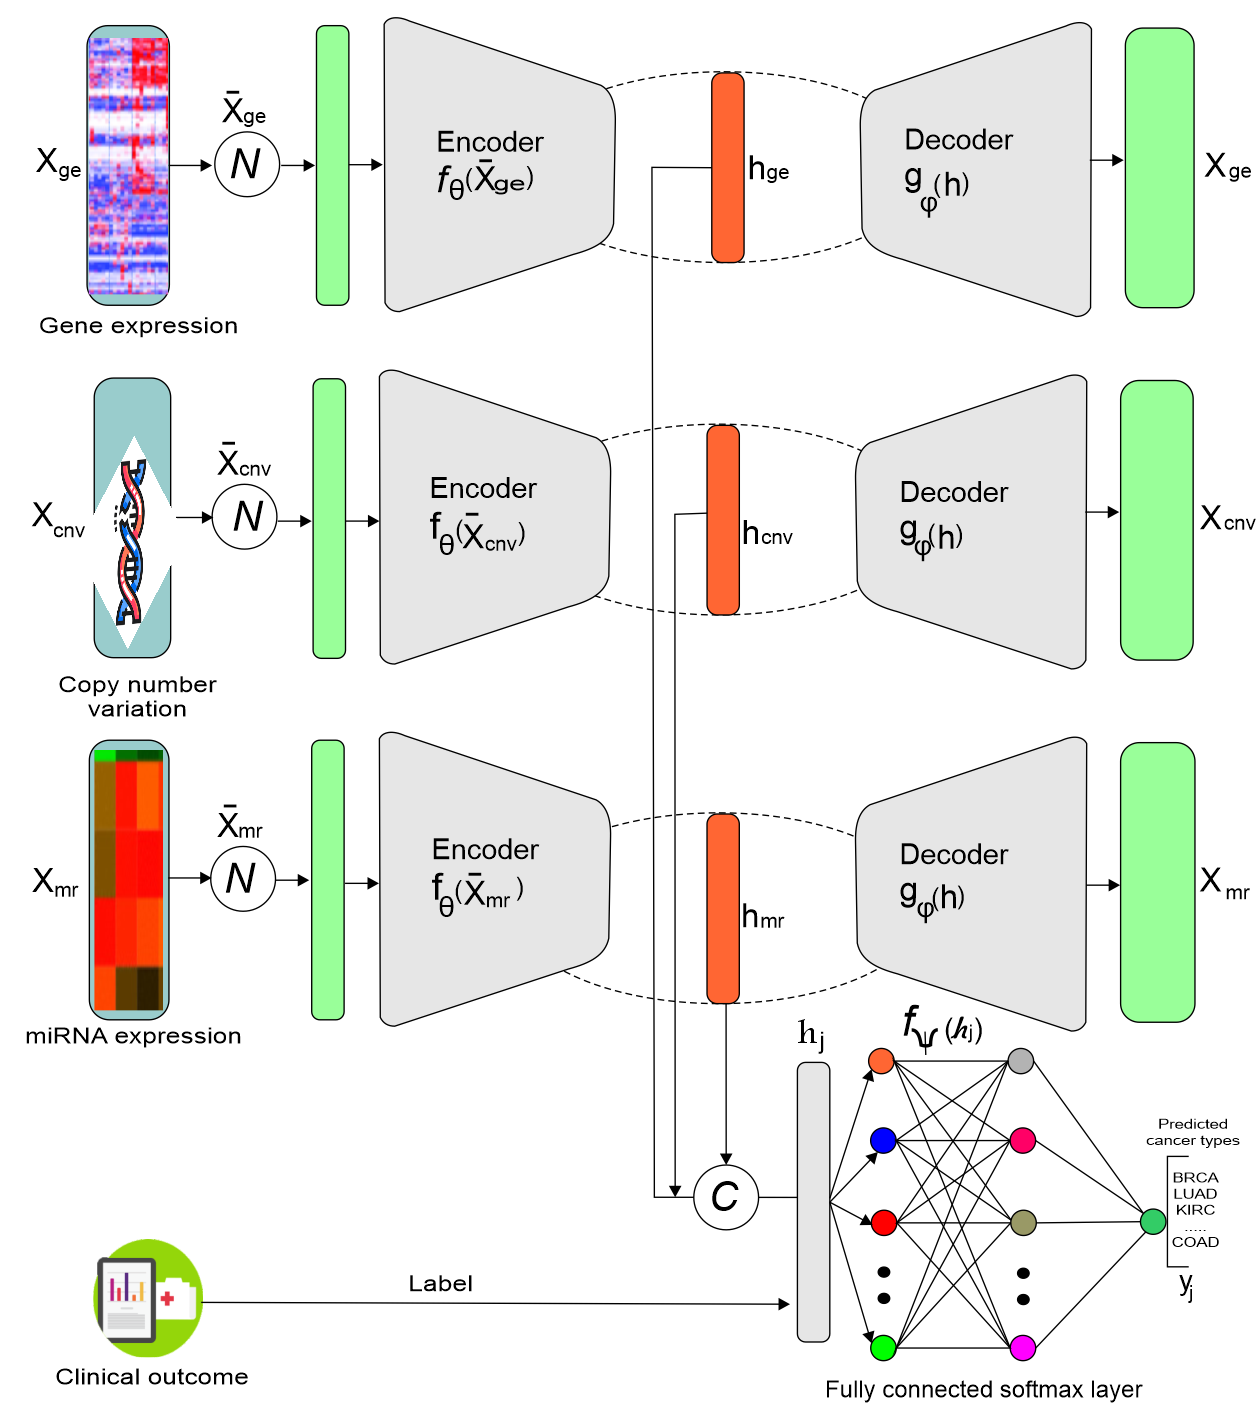
\includegraphics[scale=0.7]{images/lrc_cls.png}
		\caption{Representation learning based on LRC and classification}
        \label{fig:lrc_11}
	\end{subfigure}
	\begin{subfigure}{0.48\linewidth}
		\centering
		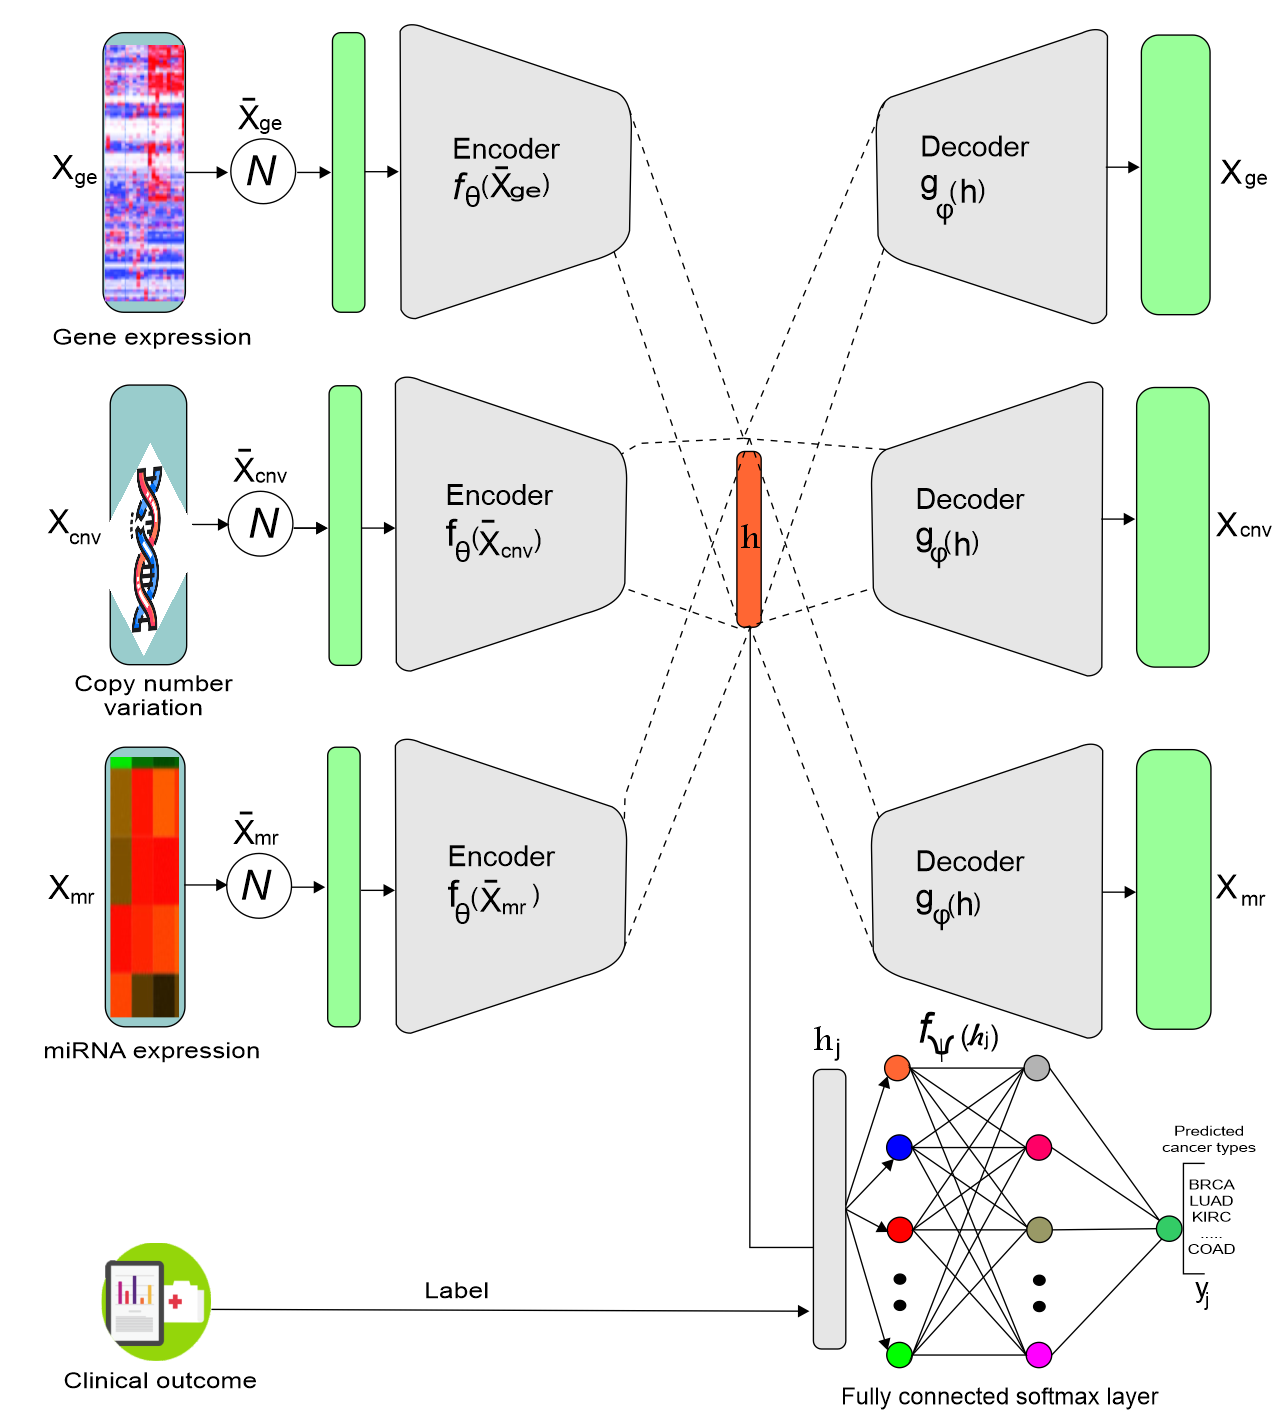
\includegraphics[scale=0.7]{images/joint_rl_cls.png}
		\caption{Representation learning based on SLR and classification}
        \label{fig:slr_11}
	\end{subfigure}
	\caption{Fusion architectures in multimodal representation learning and classification} 
	\label{fig:mm_rL_example1}
\end{sidewaysfigure*}

\subsubsection{Construction of MCAE}
Although a single and simple AE discussed in \cref{preli:AEs} can reconstruct an output similar to the original input, it cannot handle multimodality. Nevertheless, traditional supervised learning is only able to learn from the intersection of samples, which are both clean and labeled. In contrast, weights of the MCAE encoder learn from both unlabelled data, and noisy supervised data with missing modalities, leveraging as much of the available data as possible. Architecturally, MCAE is similar to a three-stage CAE: the first stage represents a particular modality for each type of data, and the second stage represents the cross-modality. CAE is trained to find a low-dimensional representation of the multimodal data, taking advantage of the information that one modality provides about another. 

\iffalse
\begin{figure*}[htp!]
	\centering
	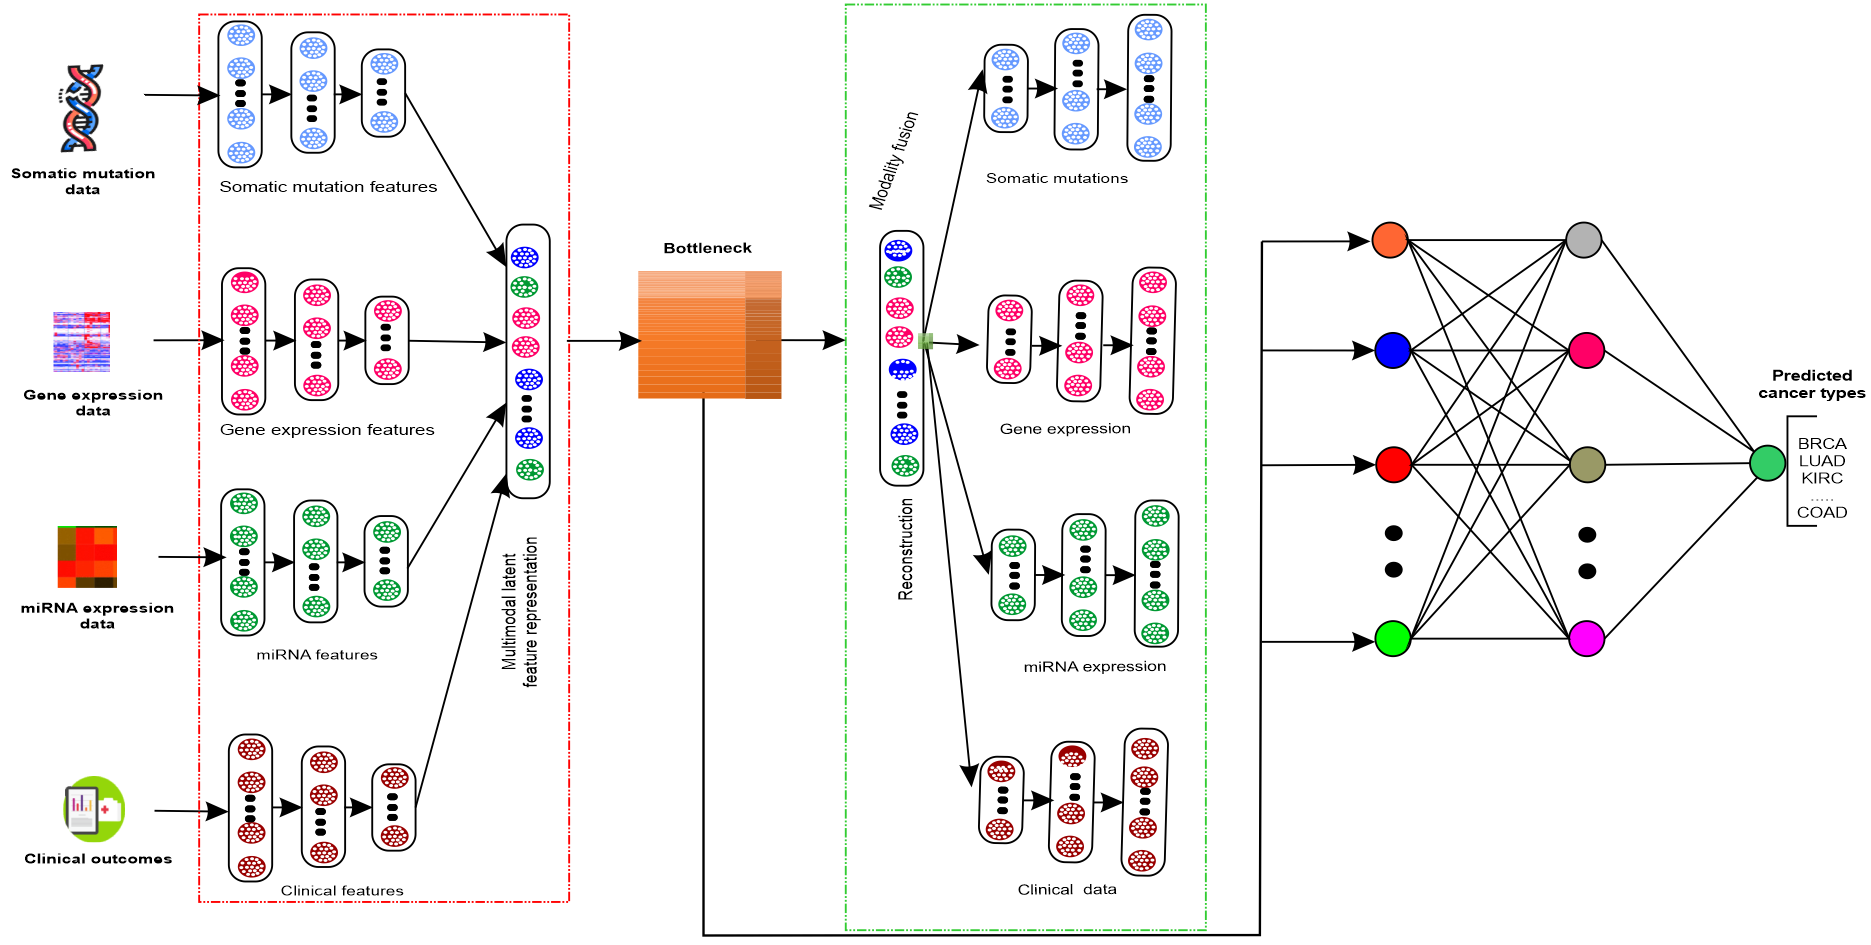
\includegraphics[width=\textwidth]{images/mcae.png}	
    \scriptsize{\caption{schematic representation of the cancer typing method based on multimodal convolutional autoencoder, which starts from taking GE, miRNA, mutations, and clinical outcomes and passing to convolutional layers before obtaining rectified conv feature maps~(with guided-backprop and GradCAM++) to pass through dense, dropout, and softmax layer}}.	
	\label{fig:mcae}
\end{figure*}
\fi 

\hspace*{3.5mm} We illustrate the construction of an MCAE as a quad-modal AE, where CNV, GE, miRNA expression, and clinical outcomes form 4 different modalities from the same patient cohorts. The individual modality CAE is not only a one-layer AE, but a multilayer and gradually shrinking CAE with the possibilities of a different number of layers for each modality, which is due to difference in dimension between modalities are pretty large. By default, MCAE fuses multiple modalities consists of a variable number of ReLU layers, which are densely connected. The cross-modality CAE is also a multilayer gradually shrinking CAE with different output layer for each prediction. However, number of layers and units per layer of the encoder and decoder networks are symmetric. The $3^{rd}$ stage is the supervised MCAE in which the decoder part is removed, and only the encoder part is utilized by adding a fully connected layer for the classification. % and regression operations. 

\subsubsection{Unsupervised pertaining of MCAE}
As shown in~\cref{fig:mm_rL_example1}, our model first embeds data of each input modality into 2D images in which each sample is reshaped into a 144$\times$144 image by zero padding around the edges and normalized to [0,255]. 
%Let's $x_m$ be the DNA methylation vector, $x_e$ is the GE vector, $x_r$ is the miRNA expression vector, and $x_c$ is the clinical data vector to hidden representations~\cite{wang2018associativemulti}.
Data $X_{i,j} \in \mathbb{R}^{D}$ for each modality $i \in \mathbb{N}$\footnote{N represents the dimensionality of the $i^{th}$ input modality} is then fed into the encoder $f_{\theta_{i}}$~(let's assume $x_m$ be the DNA methylation modality, $x_e$ is the GE modality, $x_r$ is the miRNA expression modality, and $x_c$ is the clinical data modality) in order to generate a modality specific latent representation $h_{i, j}$ as follows~\cite{mmdcae}: 

\vspace{-6mm}
\begin{align}
    h_{i,j}=f_{\theta_{i}}\left({X}_{i, j}\right)
\end{align}

\hspace*{3.5mm} where $f_\theta$ signifies trainable parameters of the encoder specific to the $i^{th}$ modality. Subsequently, the latent representation is then fed into the decoder module to reconstruct ${X}_{i, j}^{\prime}$ similar to the original input. 
%The parameters of the modality specific AE are then then trained to minimize the RL1 between the decoder’s output and the input signal, where the RL1 is similar \cref{eq:Loss1}. 
Training a single-layer autoencoder corresponds to optimizing the learning parameters to minimize the overall loss between inputs and their reconstructions, which can be defined as follows:

\vspace{-6mm}
\begin{equation}
   L_{rcae} = \min _{\theta} \sum_{i=1}^{n} \left\|x_{t}^{i}-\hat{x}_{t}^{i}\right\|^{2}+\left\|x_{v}^{i}-\hat{x}_{v}^{i}\right\|^{2}+\left\|x_{a}^{i}-\hat{x}_{a}^{i}\right\|^{2}
   \label{eq:recons_loss_2}
\end{equation}

\hspace*{3.5mm} where $i$ denotes the $i^{th}$ feature. The latent representations of all modalities are further concatenated into a single representation $h_{i,j} \in \mathbb{R}^{d}$. To create the shared representation, we ensured that all latent representations have the same dimensionality, s.t. $\forall i \in\{0,1, \ldots, n\}, d_{i}=$ $\eta \in \mathbb{N}$~\cite{mmdcae}. Similar to the architecture depicted in \cref{fig:lrc_1}, we employ LRC from all input modalities. The resulting concatenated generates a single vector $u=\left[u_{0}, u_{1}, \ldots, u_{n}\right] \in[-1,1]^{(n+1) \eta}$, where the weights of the corresponding components are generated using the softmax layer as follows~\cite{mmdcae}:

\vspace{-6mm}
\begin{align}
    \omega=\operatorname{softmax}\left(W_{\omega} u+b_{\omega}\right),
\end{align}

\hspace*{3.5mm} where $\omega=\left[\omega_{0}, \omega_{1}, \ldots, \omega_{n}\right] \in[0,1]^{(n+1) \eta}$ $\left(\forall i, \omega_{i} \in[0,1]^{\eta}\right)$, and  $W_{\omega} \in$ $\mathbb{R}^{(n+1) \eta \times(n+1) \eta}$ and $b_{\omega} \in \mathbb{R}^{(n+1) \eta}$ is the trainable parameters ~\cite{mmdcae}. The final latent representation is generated through a weighted sum of all the modalities specific latent representation $\left(h_{i,j}\right)$ based on the computed weights $\left(\omega_{i}\right)$ as follows~\cite{mmdcae}: 

\vspace{-6mm}
\begin{align}
   h_{i,j}=\sum_{i=1}^{n}\left(h_{i} \odot \omega_{i}\right),
   \label{eq:mcae_latent_final}
\end{align}

\hspace*{3.5mm} where $\odot$ denotes the element-wise product and $h \in$ $\mathbb{R}^{\eta}$ is the final representation~\cite{mmdcae}, which is subsequently fed to the classifier for the classification. 

\subsubsection{Supervised training of MCAE}
The final concatenated latent representation is fed into the fully-connected layer for the classification, which is trained to optimize the categorical cross-entropy loss (see \cref{eq:cross_entropy_loss_2}). Softmax activation function is used in the output layer for the probability distribution over the classes. Overall, the parameters of the entire MCAE architecture are optimized by minimizing the following objective function~\cite{mmdcae}:

\vspace{-4mm}
\begin{align}
    {L}=\sum_{i=0}^{n} \alpha_{r} {L}_{rcae}+\alpha_{c} {L}_{ccae}
    \label{eq:sum_2}
\end{align}

\hspace*{3.5mm} where the parameters $\alpha_{rcae}$ and $\alpha_{ccae}$ are regularization weights assigned to each error function~\cite{mmdcae}. Before the training, the MCAE network parameters were initialized with Xavier initialization~\cite{xavier} and trained using first-order gradient-based optimization techniques AdaGrad. 

\subsubsection{Interpreting black-box MCAE model}
%We discuss details of the construction and training of the MCAE architecture, followed by providing explanations of the interpretability in this sub-section. 
%\Cref{fig:tsne_ge} shows the t-SNE visualization based on GE  profiles. 
Majority of the approaches based on multimodal learning directly merge the learned or latent vectors. Consequently, the learned representations from CAE are not easily interpretable, which is a very critical drawback. However, disentangling them is essential to provide insight into what features did the representations capture and what attributes of the samples are the classification based on~\cite{karimTCBB2020}. As mentioned earlier, there is not huge difference between GE, miRNA, or CNV features values. Therefore, merging them blindly could ignore subtle differences between different input modalities w.r.t feature contributions and may increase dimensions of the representation. 

\begin{sidewaysfigure*}
	\centering
	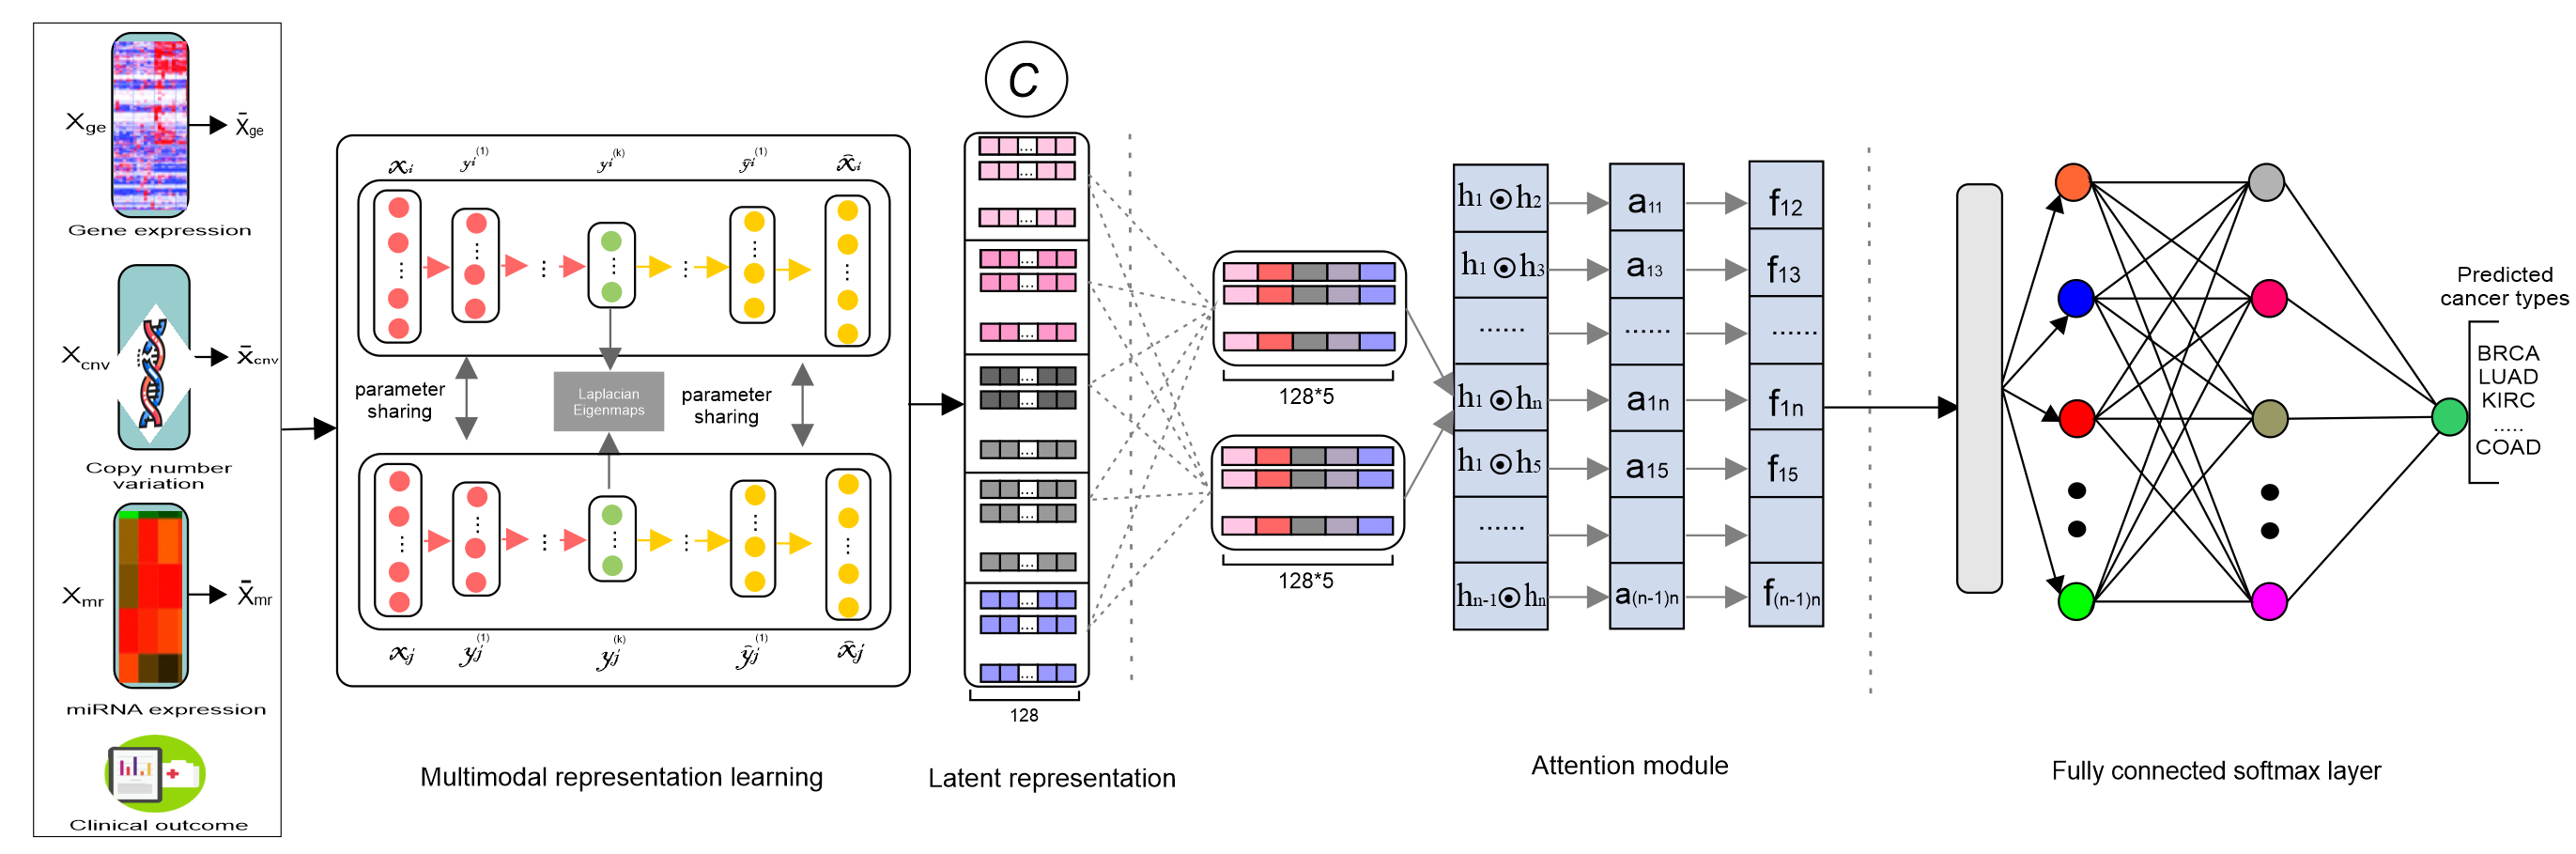
\includegraphics[scale=0.6]{images/attention.png}	\caption{The schematic representation of the attention mechanism}.	
    \vspace{-2mm}
	\label{fig:attention}
\end{sidewaysfigure*}

\hspace*{3.5mm} Unlike the unimodal CNN models, where CNN-based feature selection is performed, it is more reasonable to let the MCAE model to perform feature selection. One of the widely used techniques is called attention mechanism. Motivated by the facts that attention networks have already been applied in numerous research domains, an attention layer is added to compute important features by fusing different features and their dimensions before the actual concatenation, as shown in \cref{fig:attention}. Then, from the final concatenated vector $h_{i,j}$ in \cref{eq:mcae_latent_final} that already combined diverse information learned from three different modalities. From $K$  dimensional latent vector space, the representation is learned from the latent vectors of individual features. The resulting representation of feature $i$ can be defined as follows: 

\vspace{-6mm}
\begin{align}
    f_{i,j}=a_{i,j} \odot\left(h_{i} \odot h_{j}\right)
\end{align}
\vspace{-6mm}

\hspace*{3.5mm} where $\odot$ is the element-wise product, $a_{i,j}$ = $\left(a_{i,j,1}, a_{i,j,2}, \cdots, a_{i,j,K}\right)$ is a $K$ dimensional attention vector to reflect the different importance by fusing latent vectors $h_{i}$ and $h_{j}$. Specifically, $f_{i,j}=$ $\left(f_{1}, f_{2}, \cdots, f_{K}\right)$ and $f_{k}=a_{i,j,k} \odot\left(h_{i,k} \odot h_{j,k}\right) \cdot a_{i,j,k}$ is the attention weight assigned to $k^{th}$ dimension. The attention vector $a_{i,j}$ is calculated as follows: 
 
 \vspace{-6mm}
 \begin{align}
    a_{i, j, k}=\frac{\exp \left(\hat{a}_{i, j, k}\right)}{\sum_{m=1}^{k} \exp \left(a_{i, j, m}\right)}
\end{align}

\hspace*{3.5mm} where $\hat{a}_{i,j}=V^{T} \operatorname{ReLU}\left(W\left(Y_{i} \odot Y_{i}\right)+b\right)$ and $\operatorname{ReLU}$ is ReLU activation function, $b$ and $W$ are the bias vector and the weight matrix, and $V^{T}$ is the weight vector. These parameters are optimized along with deep neural network in an end-to-end way. The final outcome of the attention module takes into account the different contributions of different features w.r.t their dimensions. Output from the attention layer, i.e., multimodal features is then feed into a fully-connected layer for making the prediction. 

%\Cref{algo:hm_2} and \ref{algo:imp_area_2} depict the pseudo-codes for computing feature importance with ranking genes and identification of important areas on the HM, respectively. We averaged all the normalized HM from the same class to generate a class-specific HM inspired by Selvaraju et al.~\cite{mostavi2019convolutional,karim2019onconetexplainer}.

\iffalse
\begin{figure*}[h]
	\centering
	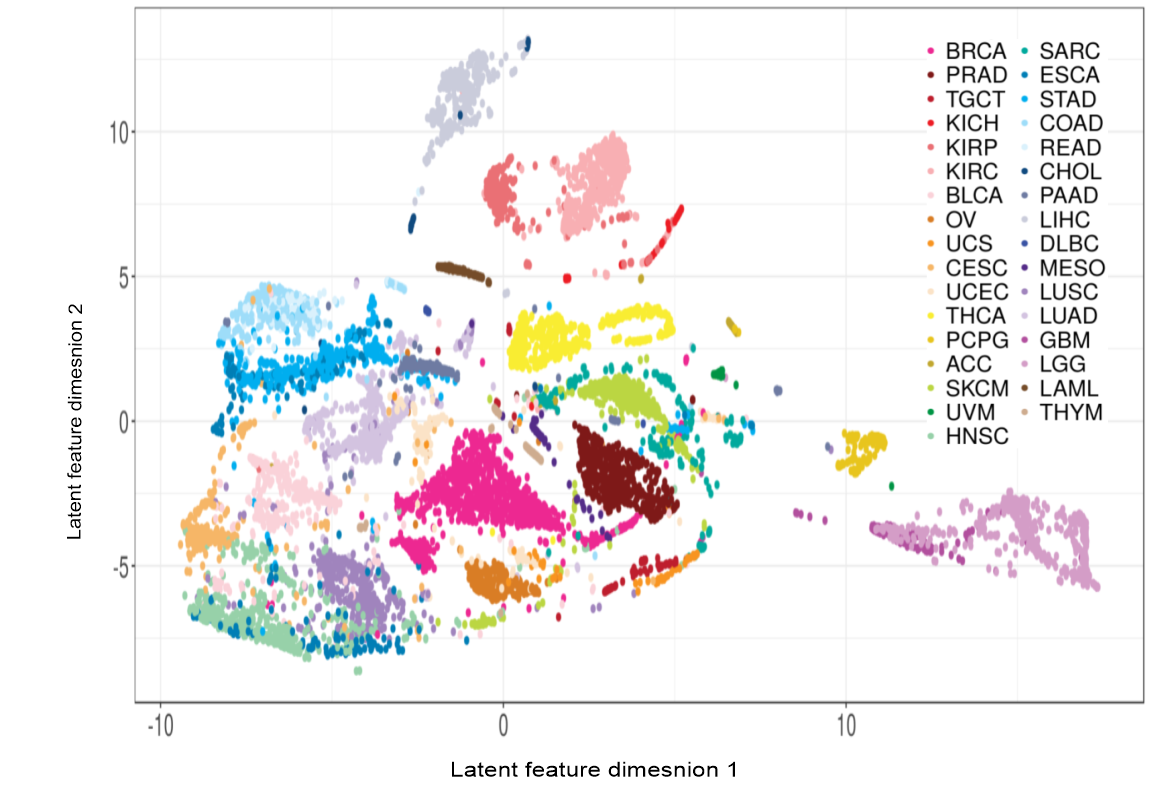
\includegraphics[width=0.85\textwidth,height=85mm]{images/ge1.png}	
    \caption{t-SNE visualization of the latent gene expression profiles.}	
	\label{fig:tsne_ge}
\end{figure*}
\fi 

%\subsubsection{Interpreting black-box MCAE model}
\hspace*{3.5mm} Since Grad-CAM++ requires all the samples to run through the network once, we let the trained CNN models set and record the activation maps in the forward pass, and the gradient maps in the back-propagation phase to collect the HM for each sample from the trained model. A higher intensity pixel represents a higher significance to the final prediction, which indicates higher importance of corresponding genes and GE values. Top genes are then selected based on the intensity rankings and MAI threshold. Since SM use true gradients, the trained weights are likely to impose a stronger bias towards specific subsets of the input pixels. Subsequently, we generate LRP and CAM-based heatmaps for each sample in the test set based on the trained CNN models, where each heatmap indicates class-discriminating pixels/features and relevance for the particular classification decision. 
%Further, SHAP is used to compute the feature importance and ranked then based on MAI. 

\iffalse
\begin{algorithm*}
\small
    \DontPrintSemicolon \SetKwInOut{Input}{Input}%
      \SetKwInOut{Output}{Output}%
      \Input{2D GE images $\mathcal{D}=(d_1,d_2,\dots,d_n)$ having ground truth~(i.e., labels) $\mathcal{L}=(l_1,l_2,\dots,l_j)$ on which a CNN model is trained for each fold $\mathcal{M}=(m_1,m_2,\dots,m_i)$ to find $k$ for top-k genes that satisfy MAI threshold.}%
      \Output{feature importance $\mathcal{F}=(f_1,i_1)(f_2,i_2),\dots,(f_n, i_n)$ and top features $\mathcal{T}$ across all images per fold per class.}%
      \BlankLine%
     \For{$\mathit{fold} \in \mathit{FOLDS}$}{
       $\mathcal{P} \leftarrow  \{\}$ \tcp*{Guided backprop for each image per fold per class}\; 
      \vspace{-4mm} 
       $\mathcal{K} \leftarrow  \{\}$ \tcp*{GradCAM++(GCAM) for all images per fold per class}\; 
      \vspace{-4mm} 
       $\mathcal{I} \leftarrow  \{\}$ \tcp*{GCAM of each image in a fold}\; 
      \vspace{-4mm} 
      $\mathcal{G} \leftarrow  \{\}$ \tcp*{GCAM for all images per fold per class}\; 
      \vspace{-4mm} 
      $\mathcal{F} \leftarrow  \{\}$ \tcp*{Feature importance of each gene per class per fold}\; 
      \vspace{-4mm} 
      $\mathcal{T} \leftarrow  \{\}$ \tcp*{Top genes and importance per class per fold}\; 
      	\vspace{-4mm} 
      	\For {$d \in \mathcal{D}$}{ 
    		$\mathcal{K} \leftarrow \mathit{gradCAM++}(m_{d}, d, l_d)$ \tcp*{GCAM of images per fold per class}\;
    		\vspace{-4mm} 
    		$\mathcal{P} \leftarrow \mathit{guidedBackprop}(m_{d}, d)$ \tcp*{Guided backprop of each image}\;
    		\vspace{-4mm} 
    		$\mathcal{I} \leftarrow \mathcal{K} * \mathcal{P}$ \tcp*{GCAM of each image}\;
    		\vspace{-4mm} 
    		$\mathcal{G} \leftarrow \mathcal{G}\cup \mathcal{I}$ \tcp*{GCAM for all the images in fold}\;
    		\vspace{-4mm} 
    	    } 
    	$\mathcal{F} \leftarrow \frac{1}{N}\sum_{i=1}^N \mathcal{G}$ \tcp*{Mean absolute impact for genes for axis=0}\;
    	\vspace{-4mm} 
    	\If{$F_i < \sigma $}{ \tcp*{If the feature importance is less than MAI}\;
    	\vspace{-4mm} 
        	$\mathcal{F} \leftarrow  F - F_i$ \tcp*{Pop off insignificant genes}\;
        	\vspace{-4mm} 
        	$\mathcal{T} \leftarrow  \operatorname{sort}_k(F)$ \tcp*{Sort and choose top genes based on MAI}\;
        	\vspace{-4mm} 
    	}
    	\textbf{Return} $\mathcal{F}, \mathcal{T}$
     }
    \caption{Computing feature importance and ranking genes}
     \label{algo:hm_2}
\end{algorithm*}

\begin{algorithm*}
\small
    \DontPrintSemicolon \SetKwInOut{Input}{Input}%
      \SetKwInOut{Output}{Output}%
      \Input{importance of current class across folds $\mathcal{F}=(f_1,\dots,f_i)$, height $h$ \& width $w$ of rectangle, \& MAI threshold $\sigma$.}%
      \Output{important areas $\mathcal{C} = (x_{1}, y_{1}),(x_{2}, y_{2}),\dots,(x_{n}, y_{n})$ in an image per fold.}%
      \BlankLine%
     \For{$\mathit{fold} \in \mathit{FOLDS}$}{
      $\mathcal{A} \leftarrow \mathit{dict}()$ \tcp*{Importance of areas}\; 
      \vspace{-4mm} 
      $\mathcal{S} \leftarrow \mathit{list}()$ \tcp*{Sorted areas by MAI}\; 
      \vspace{-4mm} 
      $\mathcal{C} \leftarrow \mathit{list}()$ \tcp*{Important areas}\; 
      \vspace{-4mm} 
      \For {$h$}{ 
        	\For {$w$}{ 
    		$area \leftarrow \mathcal{F}[h:h + \mathit{shape}[0], w:w + \mathit{shape}[1]]$ \tcp*{Area of image}\;
    		\vspace{-4mm} 
    		$impA \leftarrow 0$\tcp*{Importance of current area in the image}\;
    		\vspace{-4mm} 
    		\For {$\mathit{row} \in \mathit{area}$}{
    		%\vspace{-4mm} 
    			\For {$\mathit{imp} \in \mathit{row}$}{
    			%\vspace{-4mm} 
    			\If{$\mathit{imp} > \sigma$}{ \tcp*{If feature importance is greater than MAI}\;
    			\vspace{-4mm} 
    			    $\mathit{impA} += \mathit{imp} - \sigma$ \tcp*{Importance of area = current importance - MAI}\;
    			    \vspace{-4mm}
    			    }
    			  }
    		}
            $\mathcal{A}[\mathit{area}] = \mathit{impA}$ \tcp*{We update the importance of the area}
    	     } 
    	    }
    	$\mathcal{S} \leftarrow \operatorname{sort}(\mathcal{A}, \mathit{reverse}=\mathit{true})$ \;
    	\For {$a, i \in \mathcal{S}$}{
    	\If{$a \cap i = \empty$}{ \tcp*{Non-intersecting area with important areas}\;
    		\vspace{-4mm} 
        	$\mathcal{C} \leftarrow \mathcal{C}  \cup a$ \tcp*{It's a new important area added to the list}\;
        		\vspace{-4mm} 
    	}}
    	\textbf{Return} $\mathcal{C}$
     }
     \caption{Identification of important areas}
     \label{algo:imp_area_2}
\end{algorithm*}
\fi 
 %The idea is also to find the most important biomarkers by ranking them based on MAI threshold. 

%\todo[inline]{update}
\hspace*{3.5mm} In a previous approach~\cite{karim2019onconetexplainer}, we calculate the output gradient classes w.r.t a small change in GE, where we consider the positive values of these changes are important in the inputs. While generating SM, we fed each sample into the model to construct an interpretation map. Subsequently, we summarized each cancer type by averaging across all samples of the class and constructed a gene-effect matrix for 33 cancer types that contains gene-effect scores ranging [0,1] with 1s have maximum effect and 0 to no effect. Similar to literature~\cite{mostavi2019convolutional}, a gene with a gene-effect score greater than 0.6 was defined as a marker gene.
%In contrast, 
%Shapley values are used to calculate the importance of a feature by comparing what a model predicts with and without a feature from all possible combinations of all the features in the dataset.% as described in \cref{subsubsec:FI_shap}. 
%Shapley values are used to calculate the importance of a feature by comparing what a model predicts with and without a feature from all possible combinations of $n$ features in the dataset $S$. Given a GE value of feature $i \in S$, SHAP calculates the prediction $p$ of the model with $i$, followed by Shapely value $\phi$ calculation as follows~\cite{NIPS2017_7062}. 

\iffalse
\begin{align}
    \phi_{i}(p)=\sum_{S \subseteq N / i} \frac{|S| !(n-|S|-1) !}{n !}(p(S \cup i)-p(S))
    \label{eq:shap}
\end{align}
\fi 

%\hspace*{3.5mm} However, since the order in which a model sees features can affect the predictions, this computation is repeated in all possible orders to compare the features fairly. Feature that have no effect on the predicted value are expected to produce a Shapley value of 0. However, if two features contribute equally to the prediction, the Shapley values should be the same~\cite{NIPS2017_7062}. 

\section{Experiments}\label{chapter_5:results} 
In this section, we discuss the evaluation results, both quantitatively and qualitatively. Besides, a comparative analysis with state-of-the-art approaches is provided. 

\subsection{Experiment setup}
%All the programs were written in Python\footnote{\url{https://github.com/rezacsedu/XAI_Cancer_Prediction}}. The software stack consists of scikit-learn and Keras with TensorFlow backend. The network was trained on an Nvidia GTX 1080i GPU with CUDA and cuDNN enabled to make the overall pipeline faster. 
%Further, since an appropriate selection of hyperparameters can have a huge impact on the performance of a deep architecture, we perform the hyperparameter optimization through a random search and 5-fold cross-validation tests. In each of 5 runs, 70\% of the data is used for the training, 30\% for the evaluation, while 10\% of the training set is used for validation of the networks to optimize the cross-entropy loss based on the best learning rate, batch size, number of filters, kernel size, and dropout/Gaussian noise probability. 
Each network is trained for 500 epochs, in a similar setting of cosine annealing cycling, by setting batch size to $128$. The activity regularization term of \cref{eq:recons_loss} is set between $\lambda=[0.001, 0.005]$, while the regularization weights of the loss functions in \cref{eq:sum} are set as  $\alpha_{0}=\alpha_{1}=\alpha_{2}=0.1$, and $\alpha_{c}$=0.25. %The weight of the classifier's loss function is set greater than the others to focus more on the classification performance of the whole architecture. 
Further, the effect of minor noise~(by leveraging Gaussian noise layer) and dropout regularization are  observed. Gaussian noise parameters are empirically set to a standard deviation of 0.1 and a mean of 0. 

\hspace*{3.5mm} Results based on random hyperparameters search and 5-fold cross-validation are reported with macro-averaged precision and recall. Further, since classes are imbalanced, Matthias correlation coefficient~(MCC) scores were reported. We did not report F1-scores since it is significant only when precision and recall are very different. Thus, it is important for cancer diagnosis to have both high precision and high recall~\cite{naulaerts2017precision}, results with very different precision and recall are not useful in cancer diagnosing and tumor type identification. 
%Hence, we did not report F1-scores. 
When we create snapshots, we set the number of epochs to 200, maximum LR to 1.0, and the number of cycles to 20, giving 20 snapshots for each model. For 4 different architectures~(vanilla CNN, VGG16, $MCAE_{lrc}$, and $MCAE_{slr}$), we get 80 snapshot models in total, on which we construct the ensemble. Two best snapshot models are then used for the decision visualization and evaluations. 

\subsection{Performance analysis: single modality}
The average accuracy obtained was 89.75\% and 96.25\% using CNN and VGG16 models, respectively. However, since the classes are imbalanced, only the accuracy will give a very distorted estimation of the cancer types. Thus, we report the class-specific classification reports along with the corresponding MCC scores in \cref{table:class_specific}. As can be seen, precision and recall for the majority cancer types were high and for these the VGG16 model performs mostly better. Notably, the VGG16 model classifies BRCA, UCEC, LUAD, HNSC, LUSC, THCA, PRAD, BLCA, STAD, KIRC, LIHC, COAD, CESC, KIRP, SARC, OV, PCPG, TGCT, GBM, READ, LAML, MESO, and DLBC cancer cases more confidently, whereas the CNN model classifies PAAD, CHOL, and UCS cancer cases more accurately. 

\begin{table*}[h]
    \caption{Class-specific performance between CNN vs. VGG16 for cancer type prediction}
      \label{table:class_specific} %RF Confusion Matrix Oncogene Subtype
        \begin{center}
        \vspace{-6mm}
        \scriptsize{
        \begin{tabular}{l|lll|lll}
        \toprule
        %\rowcolor{Gray}
        {} & \multicolumn{2}{c}{\textbf{\hspace{0.7cm} CNN~(89.75\%)}} & \multicolumn{3}{c}{ \textbf{\hspace{1.5cm} VGG16~(96.25\%)}} &  {} \\
        \textbf{Type } & \textbf{Precision} &  \textbf{Recall}  & \textbf{MCC} & \textbf{Precision} &  \textbf{Recall} & \textbf{MCC} \\\midrule%\hline
        BRCA   & {\color{red}\textbf{0.8785}} & 0.8612 & 0.7564 & {\color{red}\textbf{0.9437}} & 0.9511 & 0.8465  \\%\hline
        LGG    & 0.9254 & 0.8926 & 0.8330 & 0.9311 & 0.9402 & 0.8421  \\%\hline
        UCEC   & 0.8753 & 0.8819 & 0.7835 & 0.9562 & 0.9429 & 0.8445  \\%\hline
        LUAD   & 0.8235 & 0.8354 & 0.7136 & 0.9865 & 0.9823 & 0.8624  \\%\hline
        HNSC   & 0.8520 & 0.8743 & 0.7851 & 0.9730 & 0.9822 & 0.8765  \\%\hline
        THCA   & {\color{red}\textbf{0.8528}} & 0.8323 & 0.7275 & {\color{red}\textbf{0.9138}} & 0.9154 & 0.8125  \\%\hline
        PRAD   & {\color{red}\textbf{0.8827}} & 0.8778 & 0.7847 & {\color{red}\textbf{0.9233}} & 0.9347 & 0.8207  \\%\hline
        LUSC   & 0.8726 & 0.8634 & 0.7625 & 0.9434 & 0.9472 & 0.8524  \\%\hline
        BLCA   & 0.8956 & 0.9037 & 0.8075 & 0.9656 & 0.9537 & 0.8475  \\%\hline
        STAD   & 0.8253 & 0.8156 & 0.6932 & 0.9653 & 0.9556 & 0.8532  \\%\hline
        SKCM   & 0.8853 & 0.8711 & 0.8025 & 0.9046 & 0.9136 & 0.8168  \\%\hline
        KIRC   & 0.8967 & 0.9123 & 0.8237 & 0.9578 & 0.9689 & 0.8531  \\%\hline
        LIHC   & 0.8194 & 0.8085 & 0.6945 & 0.9572 & 0.9664 & 0.8537  \\%\hline
        COAD   & 0.8368 & 0.8245 & 0.7679 & 0.9776 & 0.9690 & 0.8514  \\%\hline
        CESC   & 0.8785 & 0.8743 & 0.7964 & 0.9873 & 0.9885 & 0.8664  \\%\hline
        KIRP   & 0.8254 & 0.8032 & 0.7043 & 0.9681 & 0.9782 & 0.8430  \\%\hline
        SARC   & 0.8753 & 0.8671 & 0.7835 & 0.9365 & 0.9435 & 0.8421 \\%\hline
        OV     & 0.8825 & 0.8733 & 0.7936 & 0.9725 & 0.9773 & 0.8262  \\%\hline
        ESCA   & {\color{cyan}\textbf{0.8913}} & 0.8719 & 0.7951 &  {\color{cyan}\textbf{0.8956}} & 0.8834 & 0.8076  \\%\hline
        PCPG   & 0.8537 & 0.8611 & 0.7875 & 0.9875 & 0.9987 & 0.8735  \\%\hline
        PAAD   & 0.9629 & 0.9567 & 0.8407 & 0.9452 & 0.9500 & 0.8325  \\%\hline
        TGCT   & 0.8736 & 0.8722 & 0.7825 & 0.9890 & 0.9724 & 0.8434  \\%\hline
        GBM    & 0.8952 & 0.8845 & 0.8075 & 0.9362 & 0.9453 & 0.8436  \\%\hline
        THYM   & 0.9255 & 0.9123 & 0.8232 & 0.9775 & 0.9678 & 0.8622  \\%\hline
        READ   & {\color{cyan}\textbf{0.6795}} & 0.6857 & 0.6225 & {\color{cyan}\textbf{0.8874}} & 0.8733 & 0.7525  \\%\hline
        LAML   & 0.8697 & 0.8567 & 0.8237 & 0.9576 & 0.9632 & 0.8513  \\%\hline
        MESO   & 0.8991 & 0.9028 & 0.8076 & 0.9534 & 0.9456 & 0.8457  \\%\hline
        UVM    & 0.8765 & 0.8623 & 0.7979 & 0.9136 & 0.9089 & 0.8184  \\%\hline
        ACC    & 0.9217 & 0.9345 & 0.8225 & 0.9623 & 0.9731 & 0.8611  \\%\hline
        KICH   & 0.9335 & 0.9475 & 0.8425 & 0.9690 & 0.9625 & 0.8439  \\%\hline
        UCS    & {\color{cyan}\textbf{0.9157}} & 0.9064 & 0.8125 & {\color{cyan}\textbf{0.8726}} & 0.8675 & 0.7869  \\%\hline
        DLBC   & 0.8678 & 0.8729 & 0.7005 & 0.9347 & 0.9421 & 0.8389  \\%\hline
        CHOL   & {\color{cyan}\textbf{0.8838}} & 0.8975 & 0.7979 & {\color{cyan}\textbf{0.8455}} & 0.8342 & 0.6821  \\%\hline
        \midrule
        %\rowcolor{LightCyan}
        \textbf{Average} &   \textbf{0.8975}    &  \textbf{0.9065} &    \textbf{0.8052}   &  \textbf{0.9625} & \textbf{0.9542} & \textbf{0.8453}\\
        \bottomrule
        \end{tabular}}
        \vspace{-4mm}
    \end{center}
\end{table*}

\begin{sidewaysfigure*}
	\centering
	\begin{subfigure}{.48\linewidth}
		\centering
		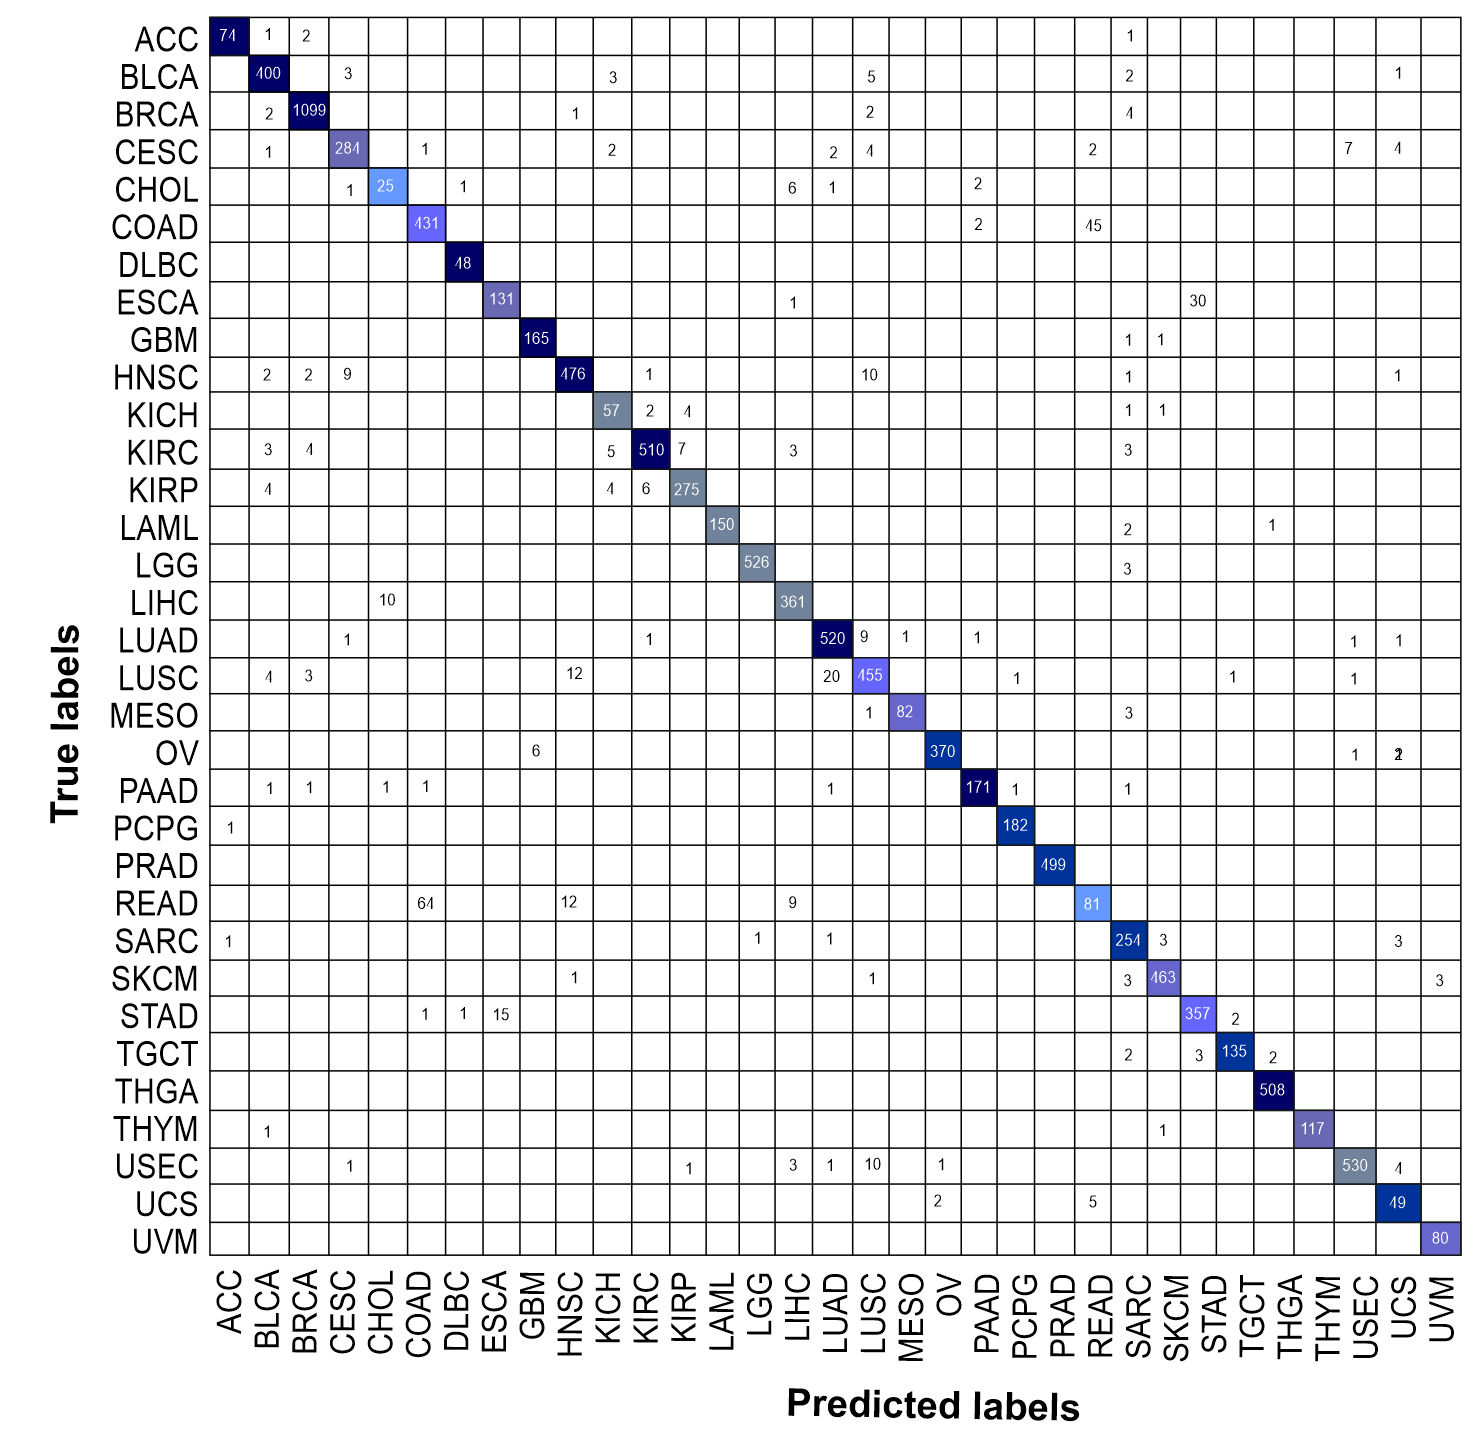
\includegraphics[width=0.8\textwidth,height=100mm]{images/conf_uni_modal.png}
		\caption{Confusion matrix}
        \label{fig:conf_cnn}
	\end{subfigure}
	\hspace{-4mm}
	\begin{subfigure}{0.48\linewidth}
		\centering
		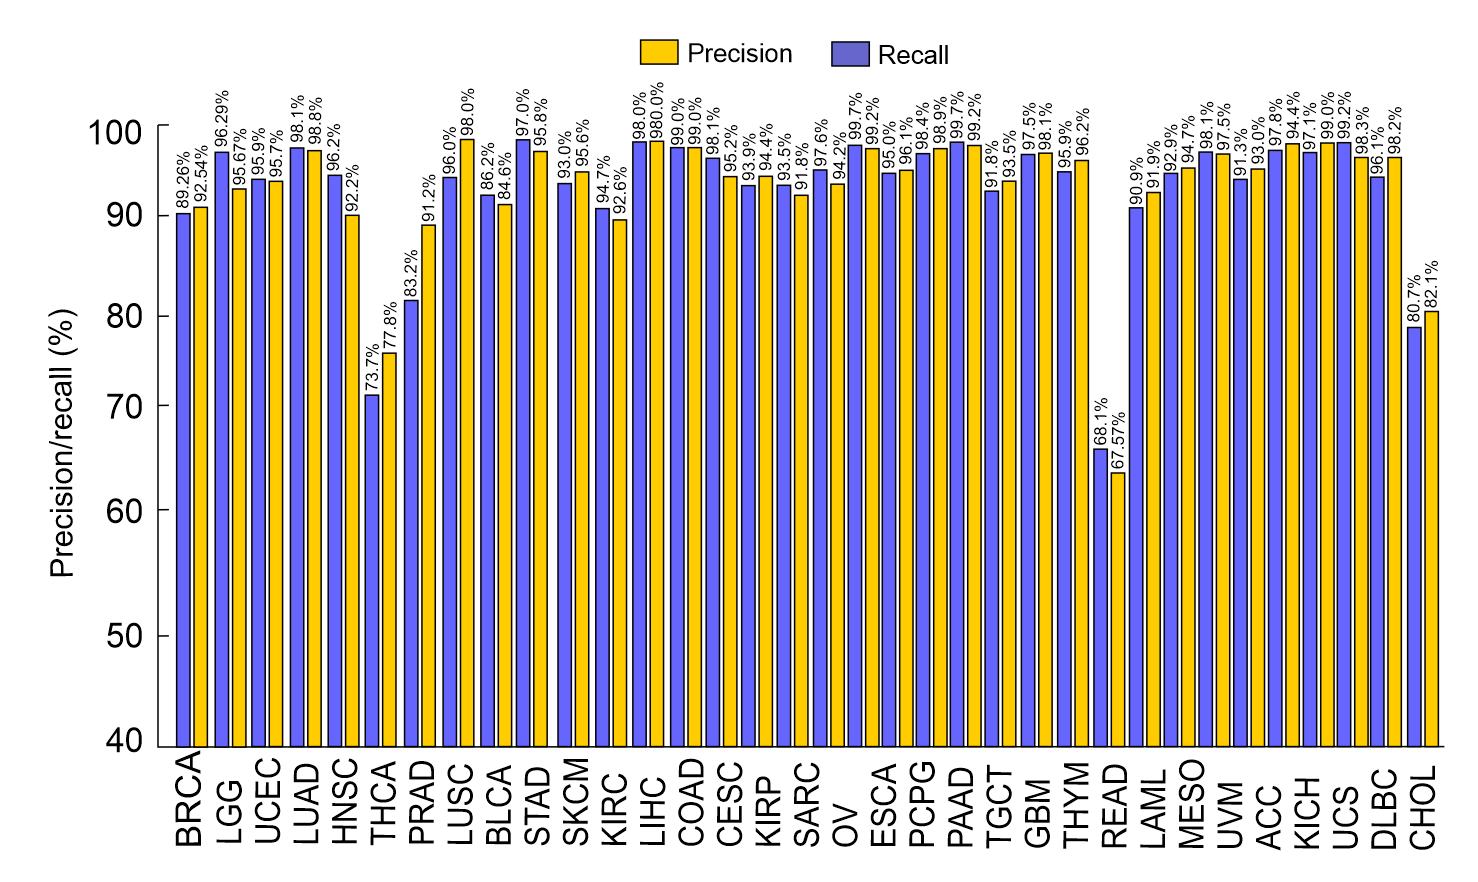
\includegraphics[width=0.9\textwidth,height=100mm]{images/pvr_value.png}
		\caption{Precision and recall}
        \label{fig:pr_vgg16}
	\end{subfigure}
	\caption{Confusion matrix, precision, and recall for VGG16 model.} 
	\label{fig:conf_precision_recall_vgg16}
	\vspace{-4mm}
\end{sidewaysfigure*}

\iffalse
\begin{figure*}[h]
\centering
	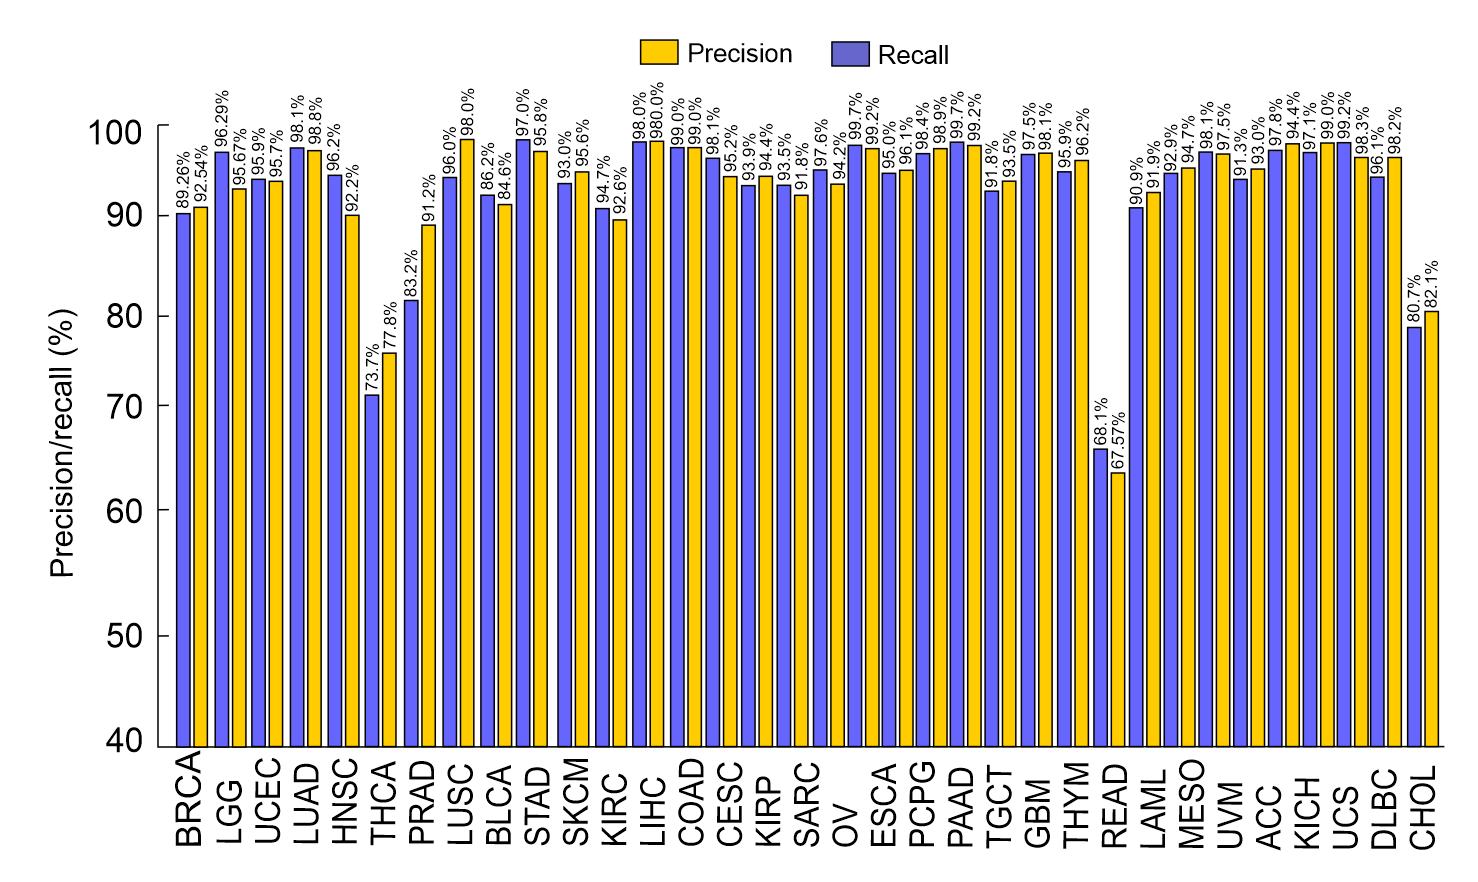
\includegraphics[scale=0.6]{images/pvr_value.png}
	\caption{Precision and recall of VGG16 model}
    \label{fig:pr_vgg16}
    \vspace{-4mm}
\end{figure*}
\fi 

\hspace*{3.5mm} The downside is that both classifiers made substantial mistakes, e.g., VGG16 could classify HNSC and LUSC tumor samples accurately in only 79\% and 81\% of the cases. On the other hand, the CNN model made more mistakes particularly on the STAD, HNSC, LUSC, and LGG tumor samples. In summary, both classifiers performed moderately well except for certain types of tumor cases such as STAD, HNSC, BLCA, THCA, UCEC, LUAD, LUSC, and LGG. The ROC curves generated by the VGG16 model 
%in \cref{fig:both_dataset} 
show that the AUC scores are consistent across the folds showing stable predictions, which shows about 5\% boost in AUC scores generated by the VGG16 model. This signifies that the predictions by the VGG16 model are much better than random guessing. 

\iffalse
\begin{figure*}[h]
    \centering
	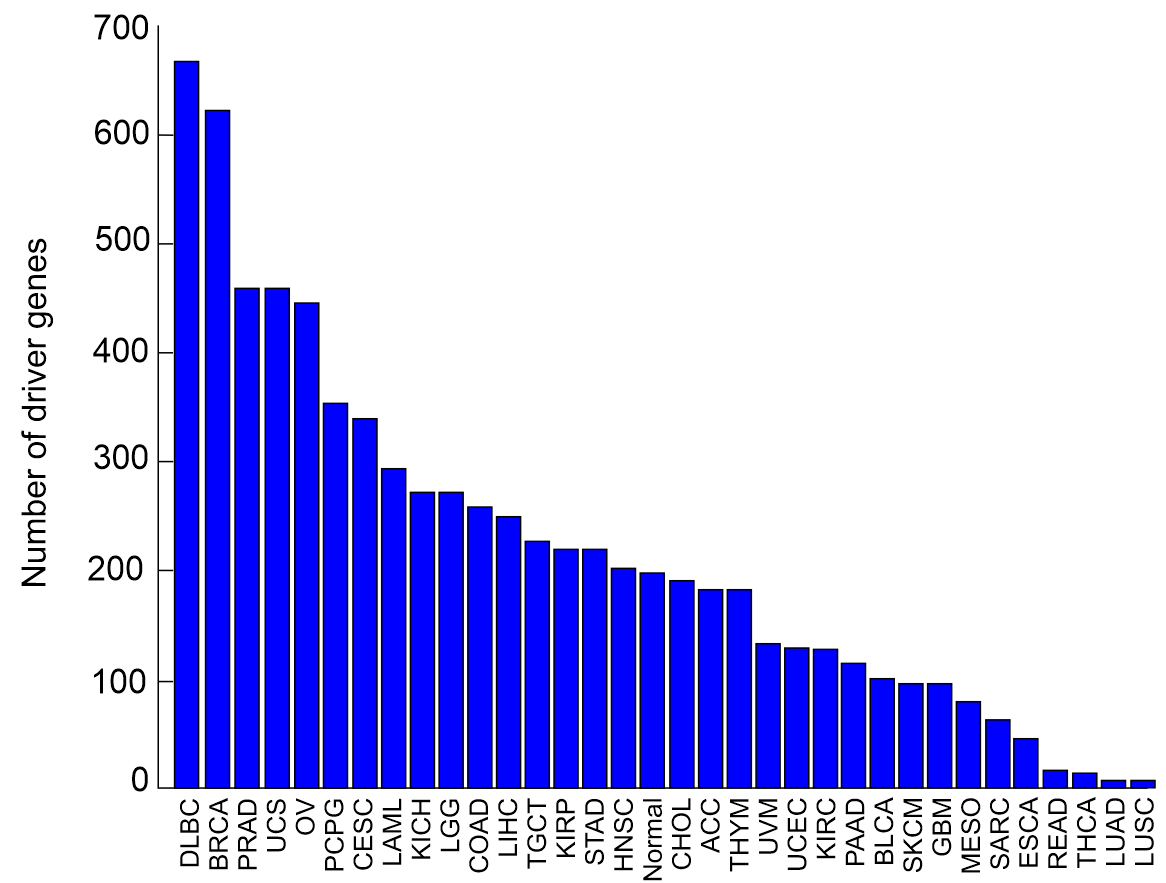
\includegraphics[width=0.8\linewidth,height=70mm]{images/driver_genes.png}
	\caption{Marker genes identified by vanilla CNN per class with a gene effect score of minimum 0.3}
    \label{fig:dg_cnn}
\end{figure*}
\begin{figure*}[h]
\centering
	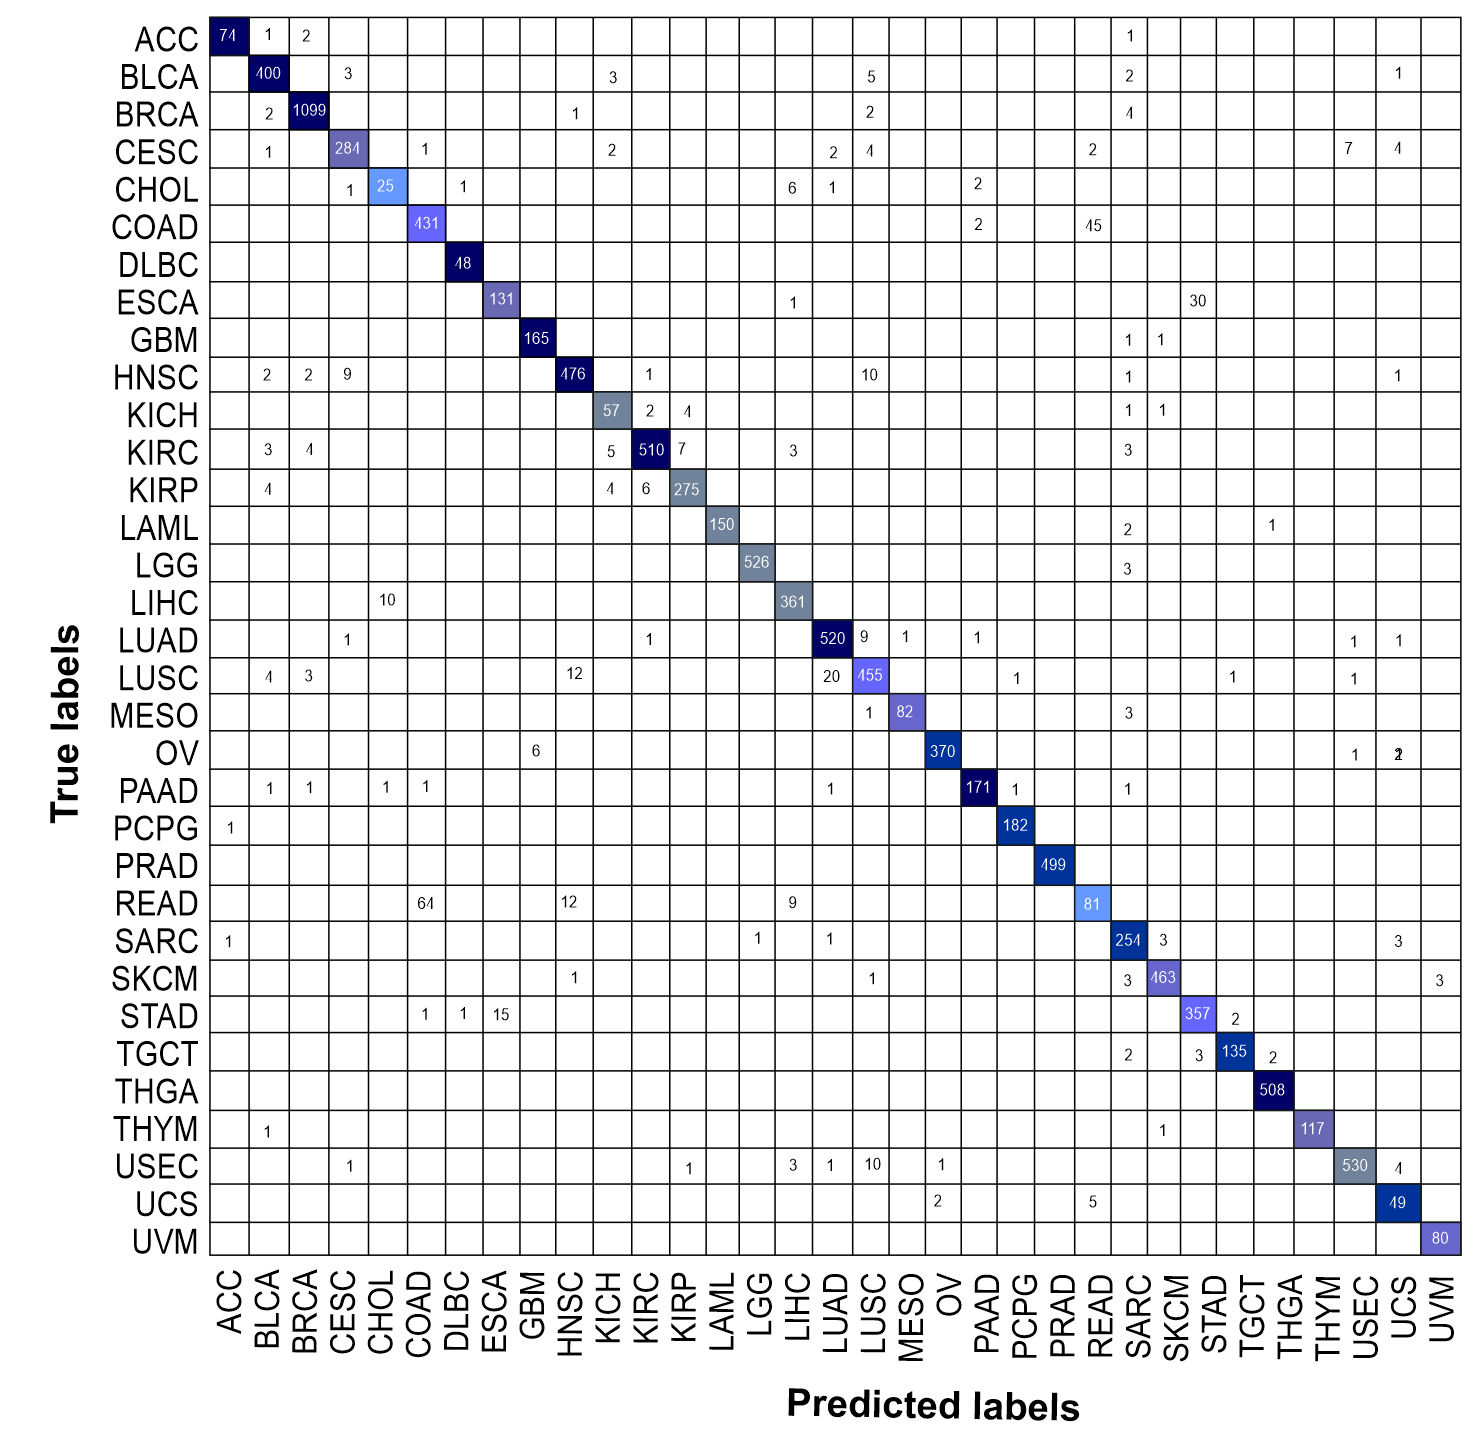
\includegraphics[scale=0.5]{images/conf_uni_modal.png}
	\caption{Confusion matrix of the VGG16 model}
    \label{fig:conf_cnn}
    \vspace{-4mm}
\end{figure*}

\begin{figure*}
	\centering
	\begin{subfigure}{.48\linewidth}
		\centering
		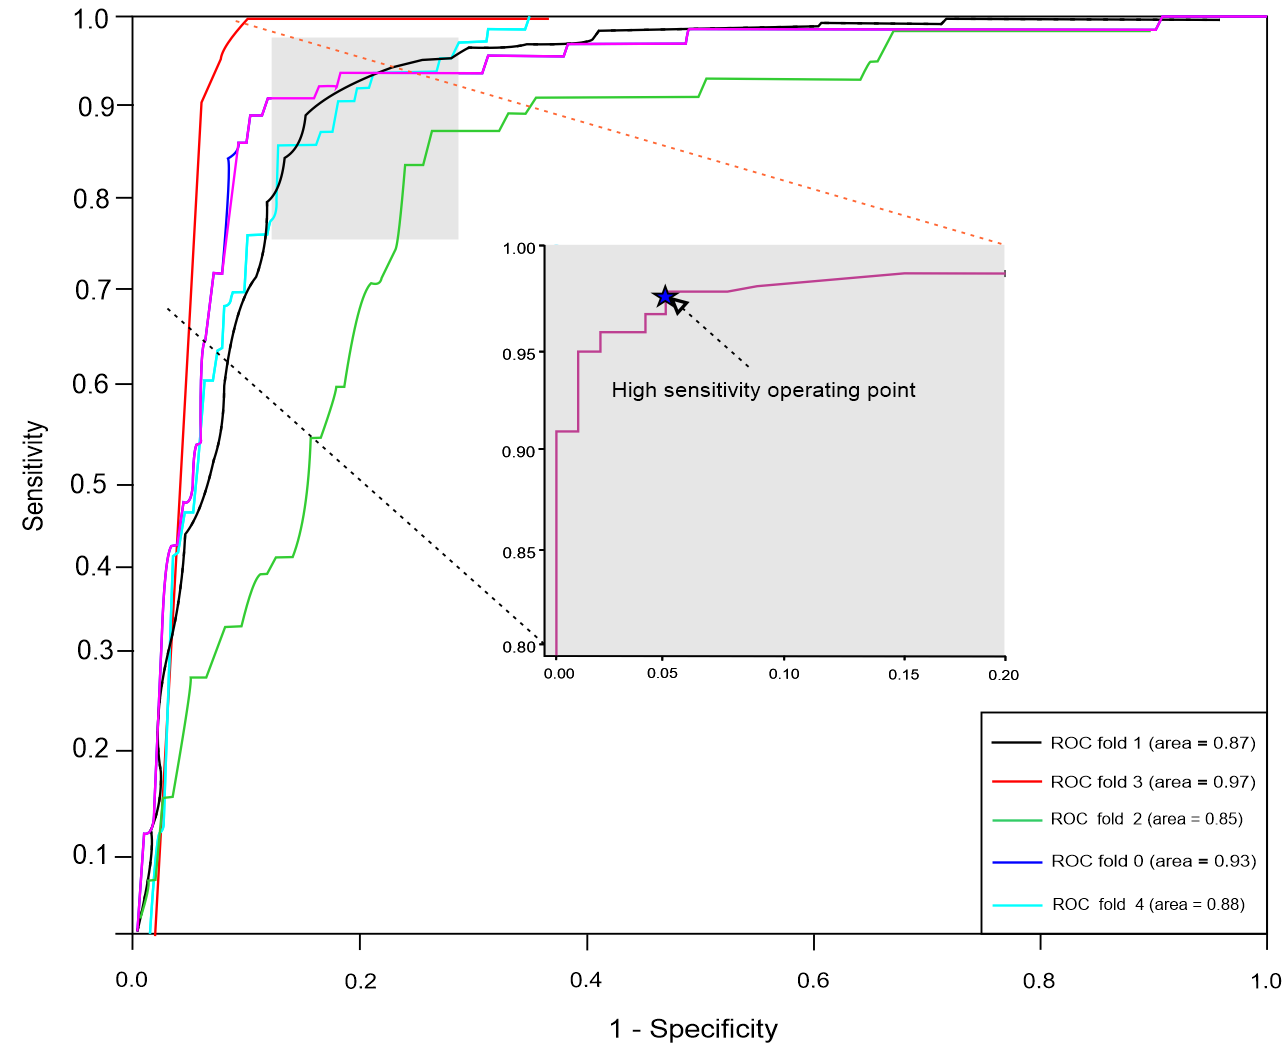
\includegraphics[scale=0.7]{images/roc_1000_genome.PNG}
		\caption{CNN}
        \label{fig:roc_cnn}
	\end{subfigure}
	\hspace{2mm}
	\begin{subfigure}{0.48\linewidth}
		\centering
		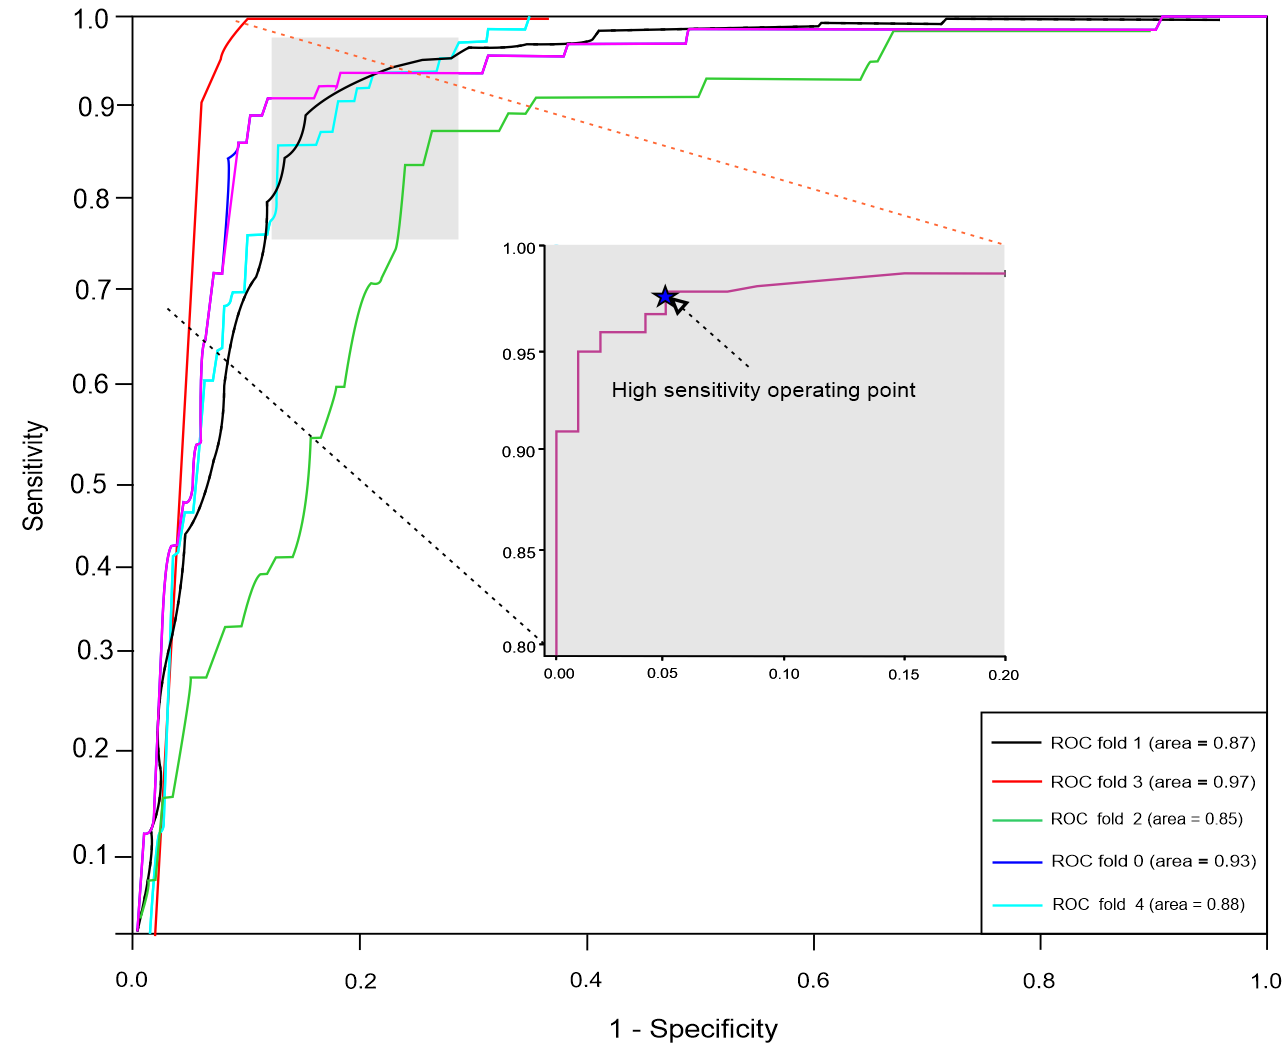
\includegraphics[scale=0.7]{images/roc_1000_genome.PNG}
		\caption{VGG16}
        \label{fig:roc_vgg16}
	\end{subfigure}
	\caption{ROC curves of the vanilla CNN and VGG16 models across folds.} 
	\label{fig:rocs}
	\vspace{-4mm}
\end{figure*}
\fi 

\hspace*{3.5mm} Further, class-specific MCC scores of VGG16 model is 4\% higher than the CNN model, which suggests that the predictions were strongly correlated with the ground truth, yielding a Pearson product-moment correlation coefficient higher than 0.70 for all the classes except for the CHOL tumor samples. The downside, however, is that both classifiers made a number of mistakes too, e.g., VGG16 can classify ESCA, READ, UCS, and CHOL tumor cases in only 89\% of the cases accurately, while the CNN model made more mistakes particularly for the READ, LUAD, LIHC, KIRP, COAD, and STAD tumor samples. Nevertheless, as is shown 17 of 23 normal classes are classified into their corresponding cancer type, where normal samples from kidney~(KICH, KIRC and KIRP), liver~(CHOL and LIHC), lung~(LUAD and LUSC) or digestive system~(ESCA and STAD) are clearly grouped together. This indicates probably the model learned to recognize tissues of origin. While we analysed the classification results of tumor samples, the major classification errors are also within kidney, lung, colon, and rectum adenocarcinomas.

\begin{sidewaysfigure*}
	\centering
	\begin{subfigure}{.48\linewidth}
		\centering
		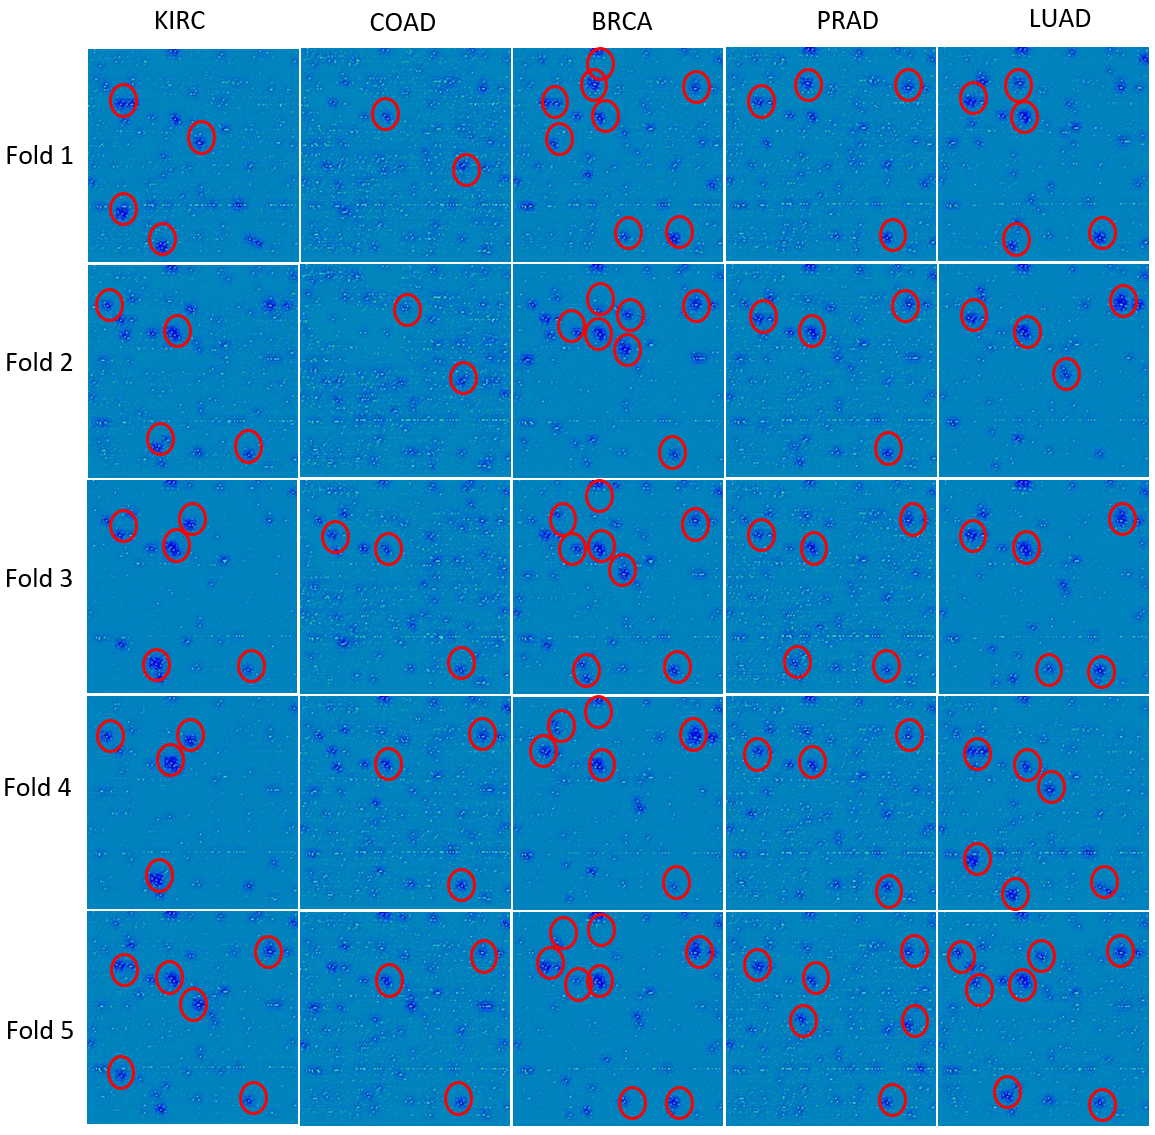
\includegraphics[scale=0.9]{images/gcam+.png}
		\caption{Grad-CAM++}
        \label{fig:hm_gcam++}
	\end{subfigure}
	%\hspace{2mm}
	\begin{subfigure}{0.48\linewidth}
		\centering
		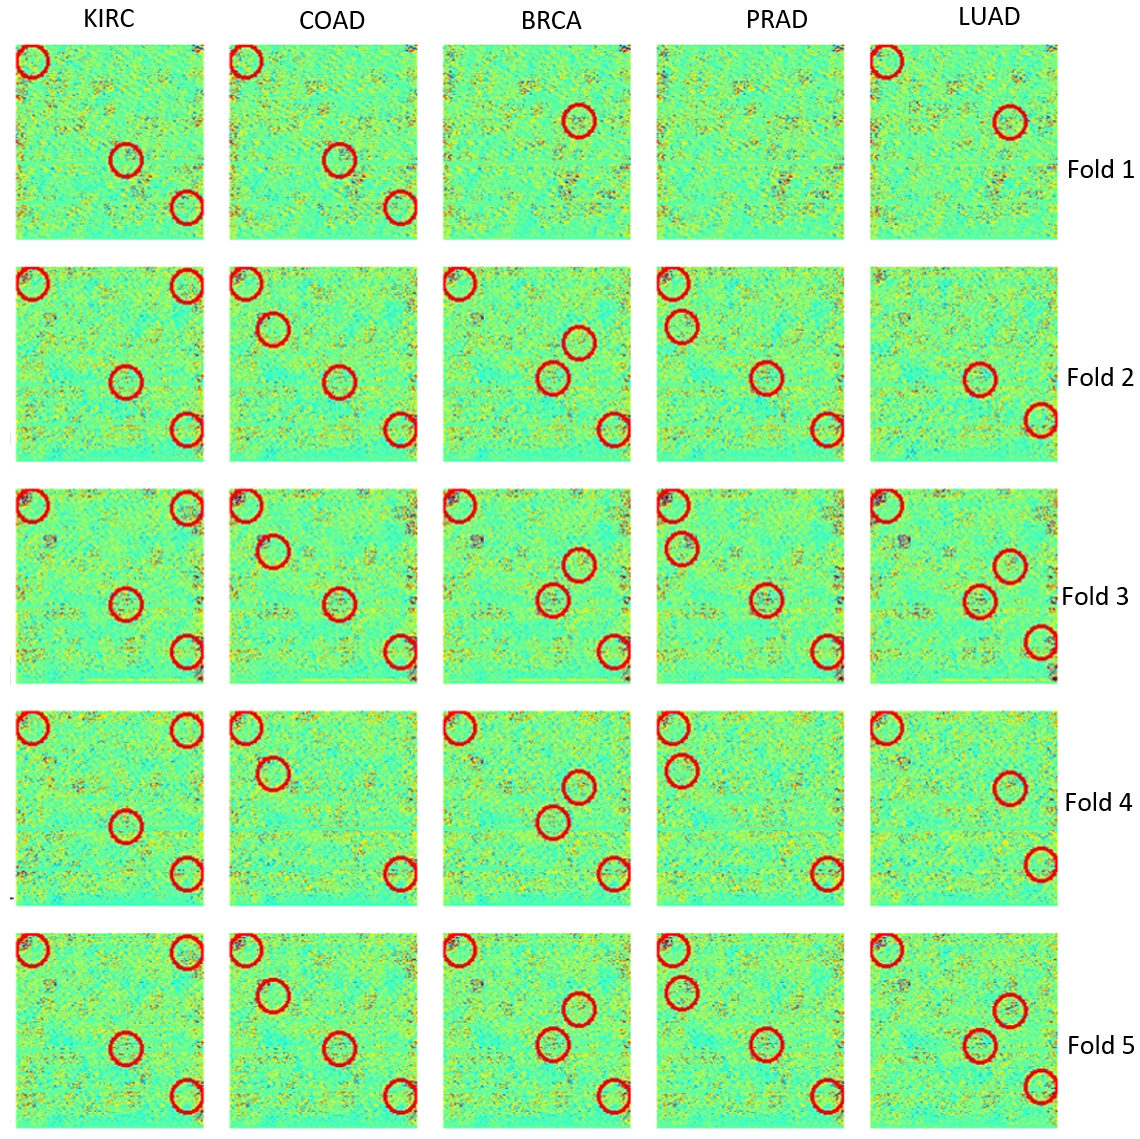
\includegraphics[scale=0.9]{images/lrp_viz.png}
		\caption{LRP}
        \label{fig:lrp}
	\end{subfigure}
	\caption[Heatmap example to mark driver biomarker for different cancer types]{Heat map examples based on Grad-CAM++ and LRP that highlight driver biomarkers for BRCA, KIRC, COAD, LUAD, and PRAD cancer types. Gene positions on 2D pixel space are marked with red circle~(genes may overlap in the marked region). Rows represent folds,  columns cancer types.} 
	\label{fig:hm_all}
	\vspace{-2mm}
\end{sidewaysfigure*}

%This part still needs to be calculated and updated 
\subsection{Performance analysis: multimodality}
The average accuracy and F1-scores by the multimodal $MCAE_{lrc}$, and $MCAE_{slr}$ models are slightly lower than the single networks. Still, $MCAE_{lrc}$ gave competitive results compared to vanilla CNN and VGG16 with a single type of input as well as $MCAE_{slr}$ for most of the cancer types. 
%as well as other best ML baselines, e.g., GBT and RF. 
In particular, GE + miRNA expression giving the best results for the classification.
%and decent results for survival rate prediction. 
Overall, both $MCAE_{lrc}$ and $MCAE_{slr}$ models better than that of MAE because of three main reasons: i) number of samples across modalities have been increased 1000 vs 10,000, ii) the reconstruction errors for both multimodal architectures based on CAE have decreased, iii) compared to ML baselines and MAE model, both $MCAE_{lrc}$ and $MCAE_{slr}$ models can learn more complex concepts from the GE + miRNA multimodal features. This results in a lower bias, which can be observed from higher training scores than the validation scores for the maximum number of samples i.e. adding more training samples does increase model generalization. 

\hspace*{3.5mm} Nevertheless, the latter two reasons helped improve the generalization by mitigating both bias and variance errors. However, we closely observed the performance of $MCAE_{lrc}$ and $MCAE_{slr}$ models. We found that $MCAE_{lrc}$ model based on LRC clearly outperforms the $MCAE_{slr}$ model. Further, we perform the Wilcoxon signed rank test with a significance level of 5\%. Then it becomes more evident from the comparison of reconstruction losses and accuracies for $MCAE_{lrc}$ and $MCAE_{slr}$ from \cref{fig:ce_multimodal_models_1} and \cref{fig:ce_multimodal_models_2}. Within each box-plot, mean and median values of the reconstruction losses are depicted with a dot and a horizontal line. As seen in \cref{fig:ce_multimodal_models_1} and \cref{fig:ce_multimodal_models_2}, $MCAE_{slr}$ model based on SLR performs worst in each and every combination of input modalities, irrespective of reconstruction loss and f1-score. 

\begin{figure*}[h]
	\centering
	\begin{subfigure}{.48\linewidth}
		\centering
		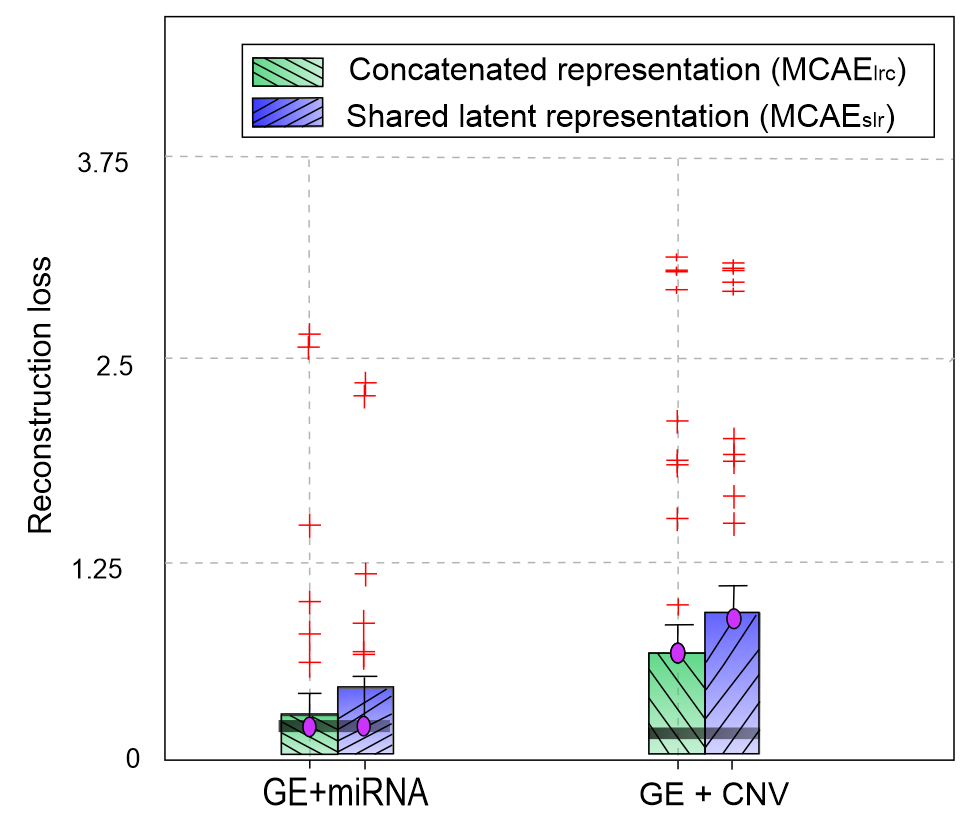
\includegraphics[width=\linewidth,height=60mm]{images/ce_mcae_1.png}
		\caption{GE+miRNA vs. GE+CNV modality}
        \label{fig:ce_ge_mirna}
	\end{subfigure}
	\begin{subfigure}{0.48\linewidth}
		\centering
		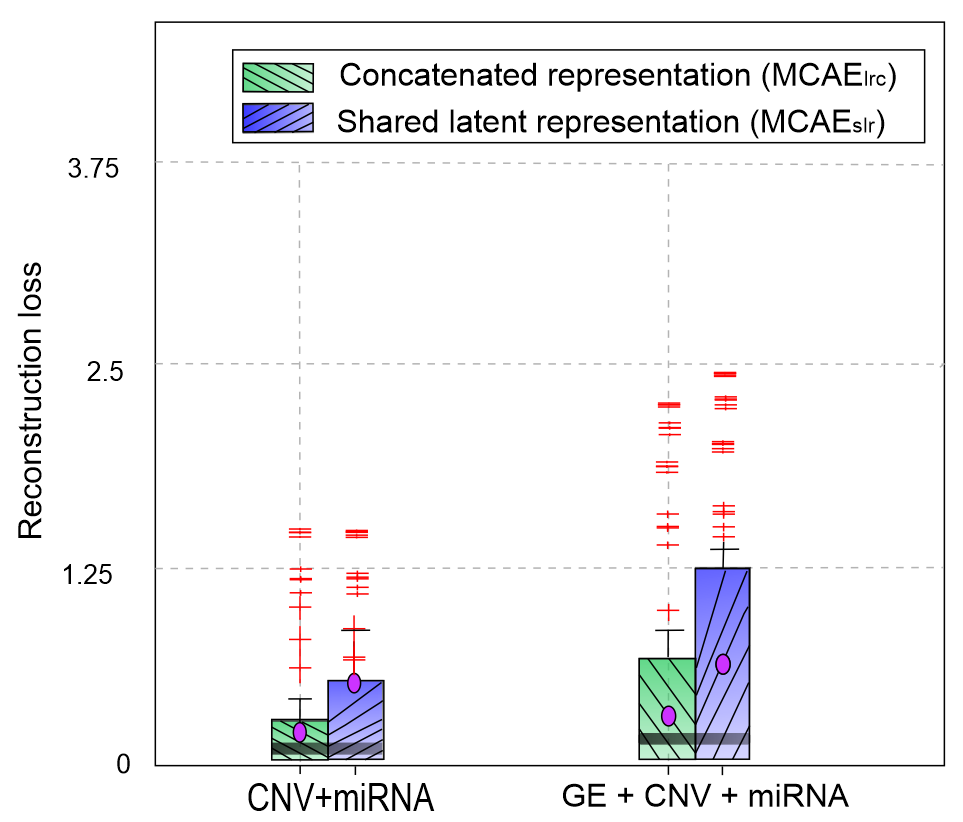
\includegraphics[width=\linewidth,height=60mm]{images/ce_mcae_2.png}
		\caption{CNV+miRNA vs. GE+CNV=miRNA modality}
        \label{fig:ce_ge_cnv}
	\end{subfigure}
	\caption{Comparison of reconstruction losses for $MCAE_{lrc}$ and $MCAE_{slr}$ during pretraining} 
	\label{fig:ce_multimodal_models_1}
\end{figure*}

\begin{figure*}[h]
	\centering
	\begin{subfigure}{.48\linewidth}
		\centering
		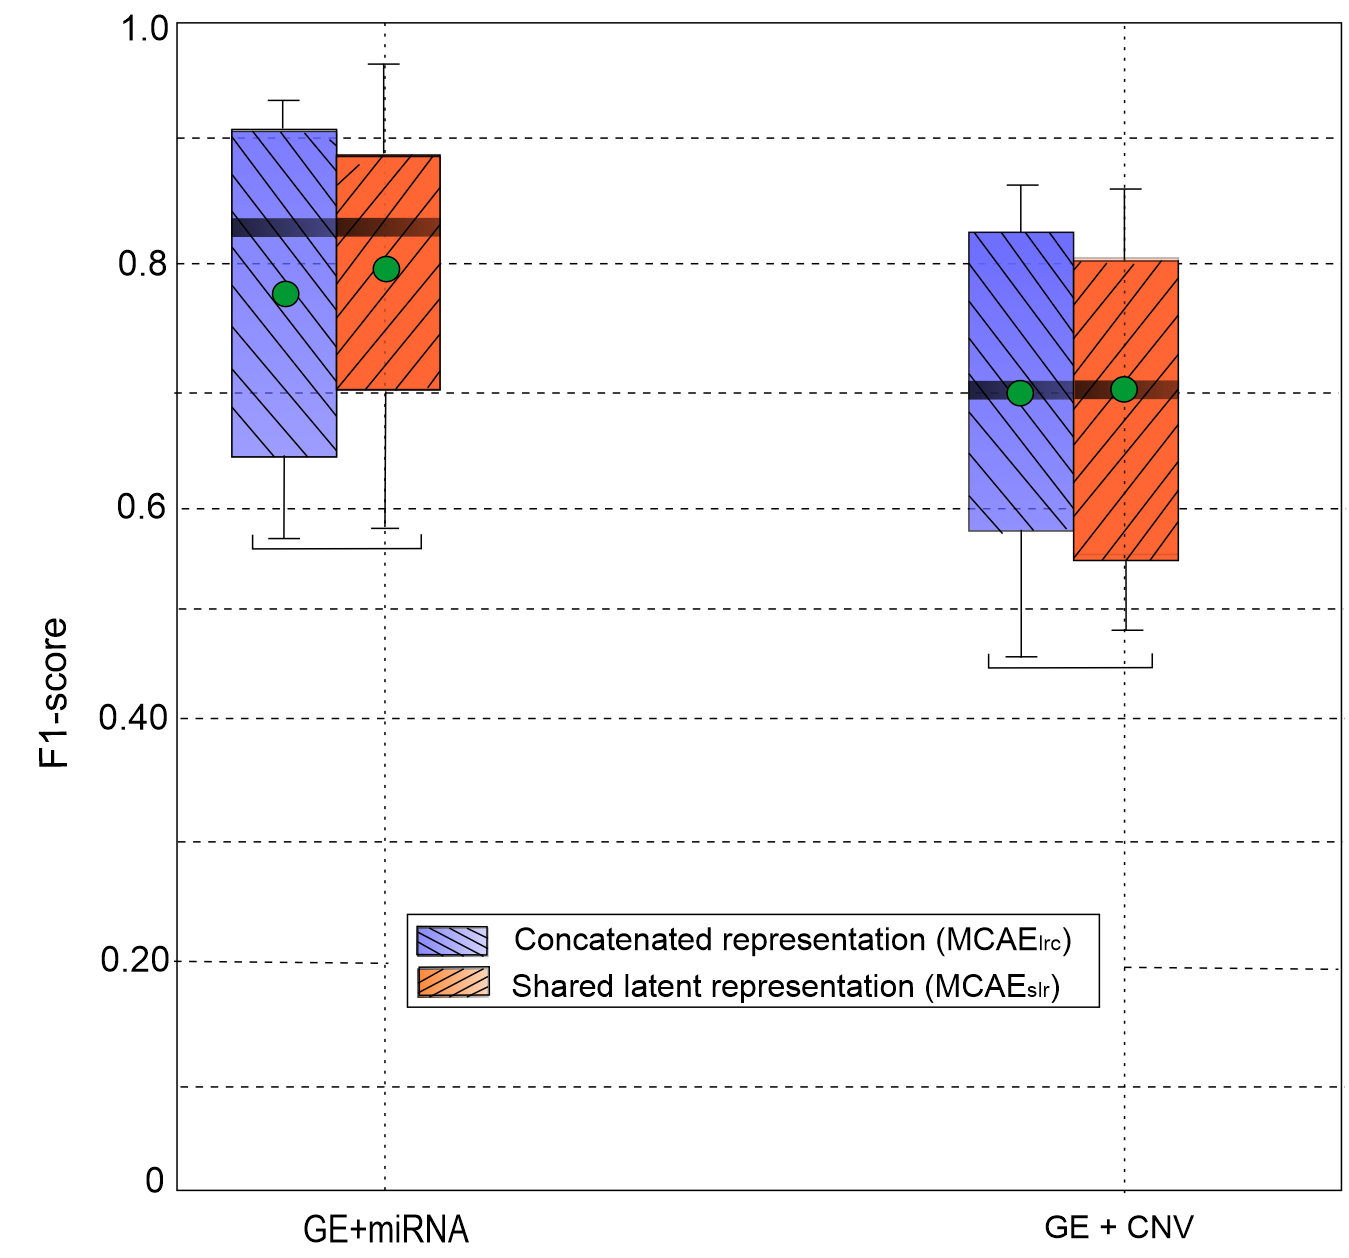
\includegraphics[width=\linewidth,height=55mm]{images/acc_mcae_1.png}
		\caption{GE+miRNA vs. GE+CNV modality}
        \label{fig:ce_ge_mirna_2}
	\end{subfigure}
	\begin{subfigure}{0.48\linewidth}
		\centering
		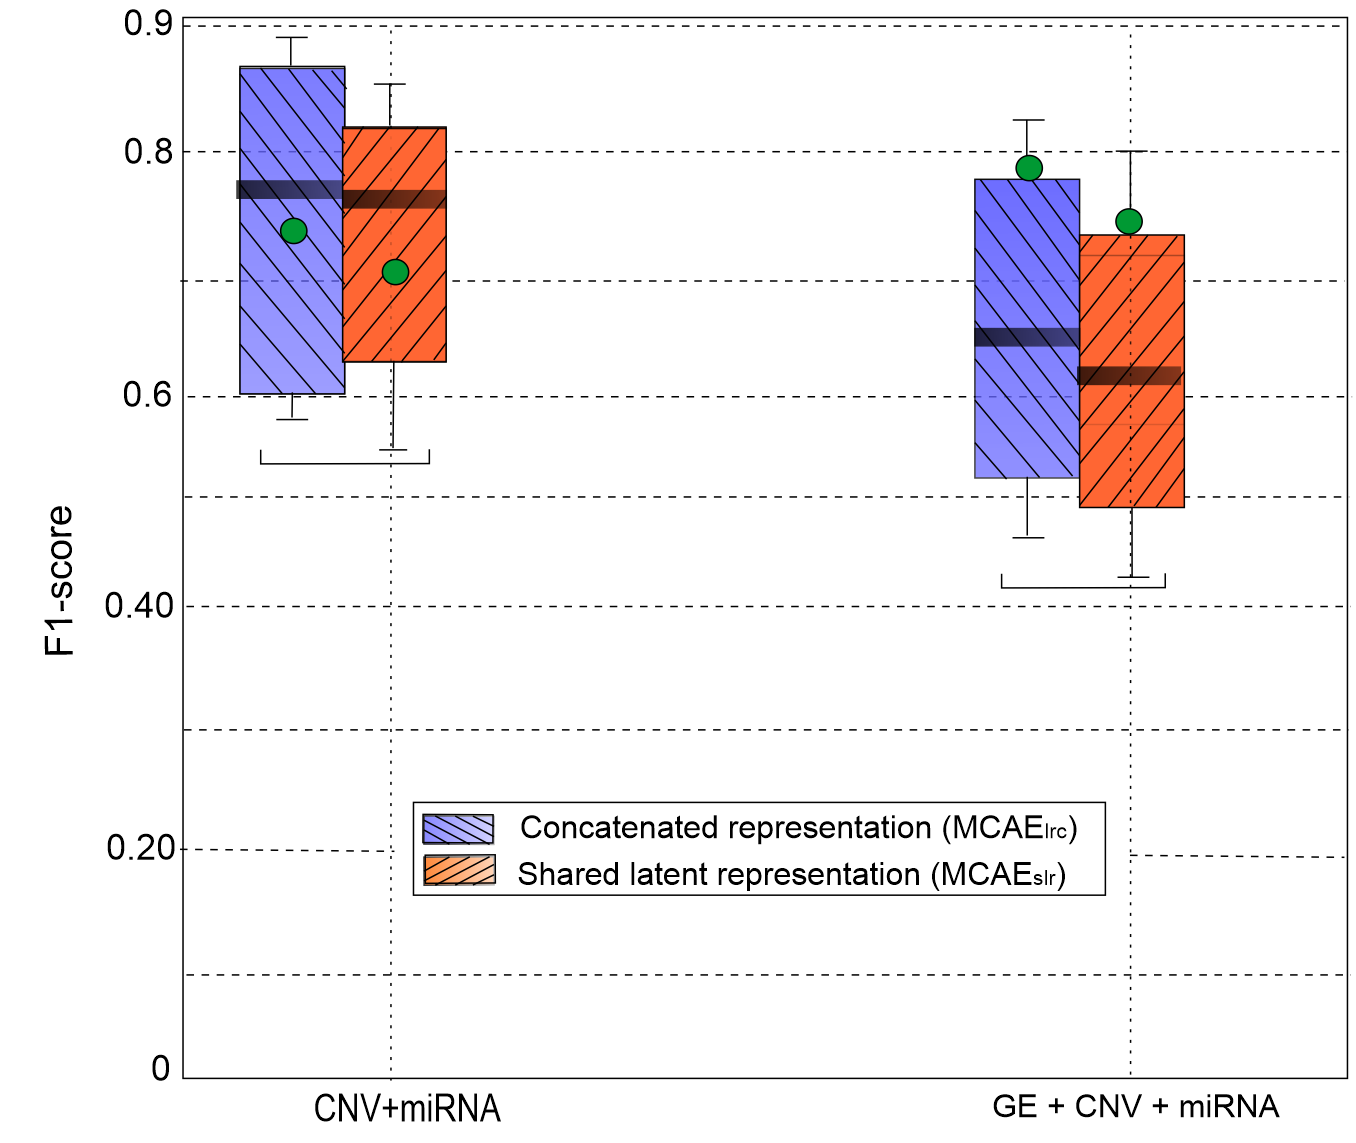
\includegraphics[width=\linewidth,height=55mm]{images/acc_mcae_2.png}
		\caption{CNV+miRNA vs. GE+CNV=miRNA modality}
        \label{fig:ce_ge_cnv_2}
	\end{subfigure}
	\caption{F1 score comparison for $MCAE_{lrc}$ and $MCAE_{slr}$ during supervised finetuning} 
	\label{fig:ce_multimodal_models_2}
\end{figure*}

\hspace*{3.5mm} In particular, the GE+miRNA input combination gave lowest reconstruction errors, whereas GE + CNV + miRNA generates the highest errors so do corresponding f1-scores. Eventually, we found that the ROC curves of the $MCAE_{lrc}$ model show that the AUC scores are consistent across the folds showing stable predictions, giving 4\% boost in AUC scores. This signifies that the predictions by the $MCAE_{lrc}$ model are clearly better than random guessing as well as $MCAE_{slr}$. It also suggests that the predictions made by the $MCAE_{lrc}$ model are strongly correlated with the ground truth, yielding a Pearson product-moment correlation coefficient higher than 0.70 for all the classes. 

\subsection{Identification of marker genes}
We identified top genes for which the change in expression has significant impact on patients. \Cref{fig:hm_all} shows examples of HM generated for each class~(each column for one cancer type) across 5 different folds. As seen, there are similarities across folds and displaying distinct and similar patterns when comparing different cancer types. Red circles highlight similar patterns, e.g., between KIRC and BRCA, and PRAD and LUAD across folds, whereas COAD shows very different patterns. Although there are differences among folds, some patterns are clearly visible. Since intensities did not follow any regular pattern, we chose top 660 genes across 33 tumor types~(top-20 genes per class) as more significant based MAI. 

\begin{figure*}[h]
    \centering
	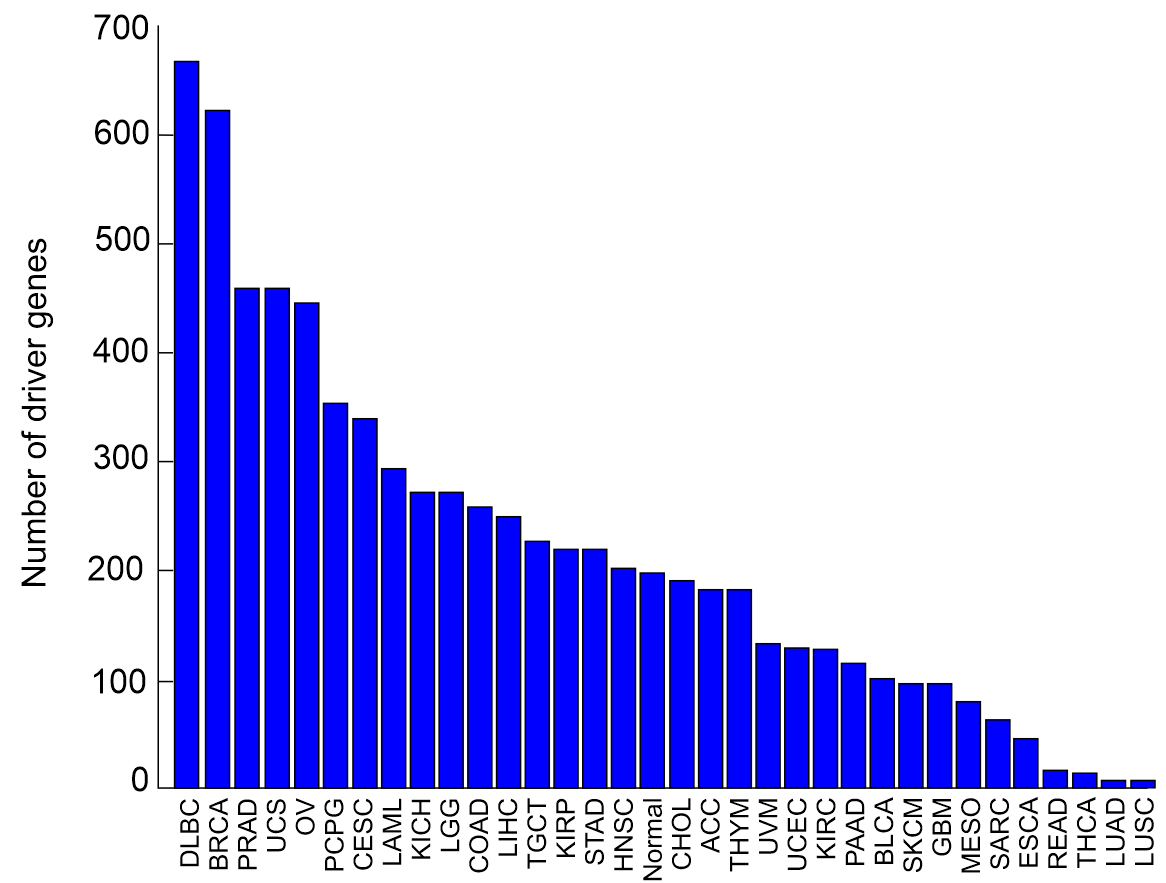
\includegraphics[scale=0.8]{images/driver_genes.png}
	\caption{Marker genes identified by $MCAE_{lrc}$ model per class with a gene effect score of $\geq$ 0.25}
    \label{fig:dg_cnn}
\end{figure*}

\hspace*{3.5mm} Since we have more than 20K protein-coding genes, our choice of 660 is still a reasonable choice, as the number of important biomarkers should be small whose GE changes are sensitive to cancer growth~\cite{zuo2019identification}. All genes in the top-20 list can thus be viewed as tumor-specific biomarkers, which contribute most toward making the predictions. As for the other 29 tumor types, only 3 genes were in the list. Further hyperparameter tuning and training of both CNN models might improve this outcome. Then we further narrowed down the list to the top-5 genes in which only 5 tumor types~(i.e., BRCA, KIRC, COAD, LUAD, and PRAD) have at least five genes with feature importance of at least 0.5 w.r.t. MAI; they are shown in \cref{table:proteinimportance} from the 20,500 protein-coding genes. 

\begin{table}
    \caption{Top-5 genes and their importance}
    \label{table:proteinimportance} %RF Confusion Matrix Oncogene Subtype
    \begin{center}
    \scriptsize
    \vspace{-6mm}
    \begin{tabular}{l|l|l|l}
        \toprule
        \textbf{Type} & \textbf{Gene} & \textbf{Gene type} & \textbf{MAI} \\ \midrule
        \multirow{5}{*}{BRCA} & PIK3CA & Oncogene & 0.78125 \\ %\cline{2-4}
        & TP53 & Protein-coding & 0.760784 \\ %\cline{2-4}
        & GATA3  & Protein-coding & 0.664706 \\ %\cline{2-4}
        & MAP3K1  & Oncogene & 0.574118 \\ %\cline{2-4}
        & APC   & Protein-coding & 0.538039 \\ \midrule
        \multirow{5}{*}{KIRC} & VHL & Oncogene & 0.596078 \\ %\cline{2-4}
        & PBRM1 & Protein-coding  & 0.560784 \\ %\cline{2-4}
        & SETD2 & Protein-coding & 0.540784 \\ %\cline{2-4}
        & PIK3CA & Oncogene & 0.531569 \\ %\cline{2-4}
        & ATM & Oncogene & 0.523137 \\ %\cline{2-4}
        \midrule
        \multirow{5}{*}{LUAD}& KRAS & Oncogene & 0.860000 \\ %\cline{2-4}
        & KEAP1 & Protein-coding & 0.820784 \\ %\cline{2-4}
        & EGFR & Oncogene & 0.764706 \\ %\cline{2-4}
        & TP53 & Protein-coding & 0.674118 \\ %\cline{2-4}
        & MLL3 & Protein-coding & 0.558039 \\ %\cline{2-4}
        \midrule
        \multirow{5}{*}{PRAD}& SPOP & Oncogene & 0.556078 \\ %\cline{2-4}
        & TP53 & Oncogene & 0.520784 \\ %\cline{2-4}
        & MED12 & Protein-coding & 0.510784 \\ %\cline{2-4}
        & PIK3CA & Protein-coding & 0.491569 \\ %\cline{2-4}
        & FOXA1 & Protein-coding & 0.453137 \\ %\cline{2-4}
        \midrule
        \multirow{5}{*}{COAD}& EPHA6 & Protein-coding & 0.756078 \\ %\cline{2-4}
        & TIMP1 & Protein-coding & 0.720784 \\ %\cline{2-4}
        & ART5 & Protein-coding & 0.680784 \\ %\cline{2-4}
        & FOXD1 & Protein-coding & 0.661569 \\ %\cline{2-4}
        & AMBN & Protein-coding & 0.563137 \\ %\cline{2-4}
        \bottomrule
        \end{tabular}
        \vspace{-4mm}
    \end{center}
\end{table}

%\subsection{Validation of top biomarkers}
\hspace*{3.5mm} To validate the findings, saturation analyses of oncogenes across 32 tumor types~(except COAD) are obtained from TumorPortal\footnote{ \url{http://www.tumorportal.org/}}~\cite{lawrence2014discovery}. Our approach makes some false identifications, as 21 out of 25 genes are validated to be correct, making only 4 false identifications. Validation for the COAD cancer follows a signature-based approach~\cite{zuo2019identification}, which was used for predicting the progression of colorectal cancer. 

\begin{sidewaysfigure*}
\centering
	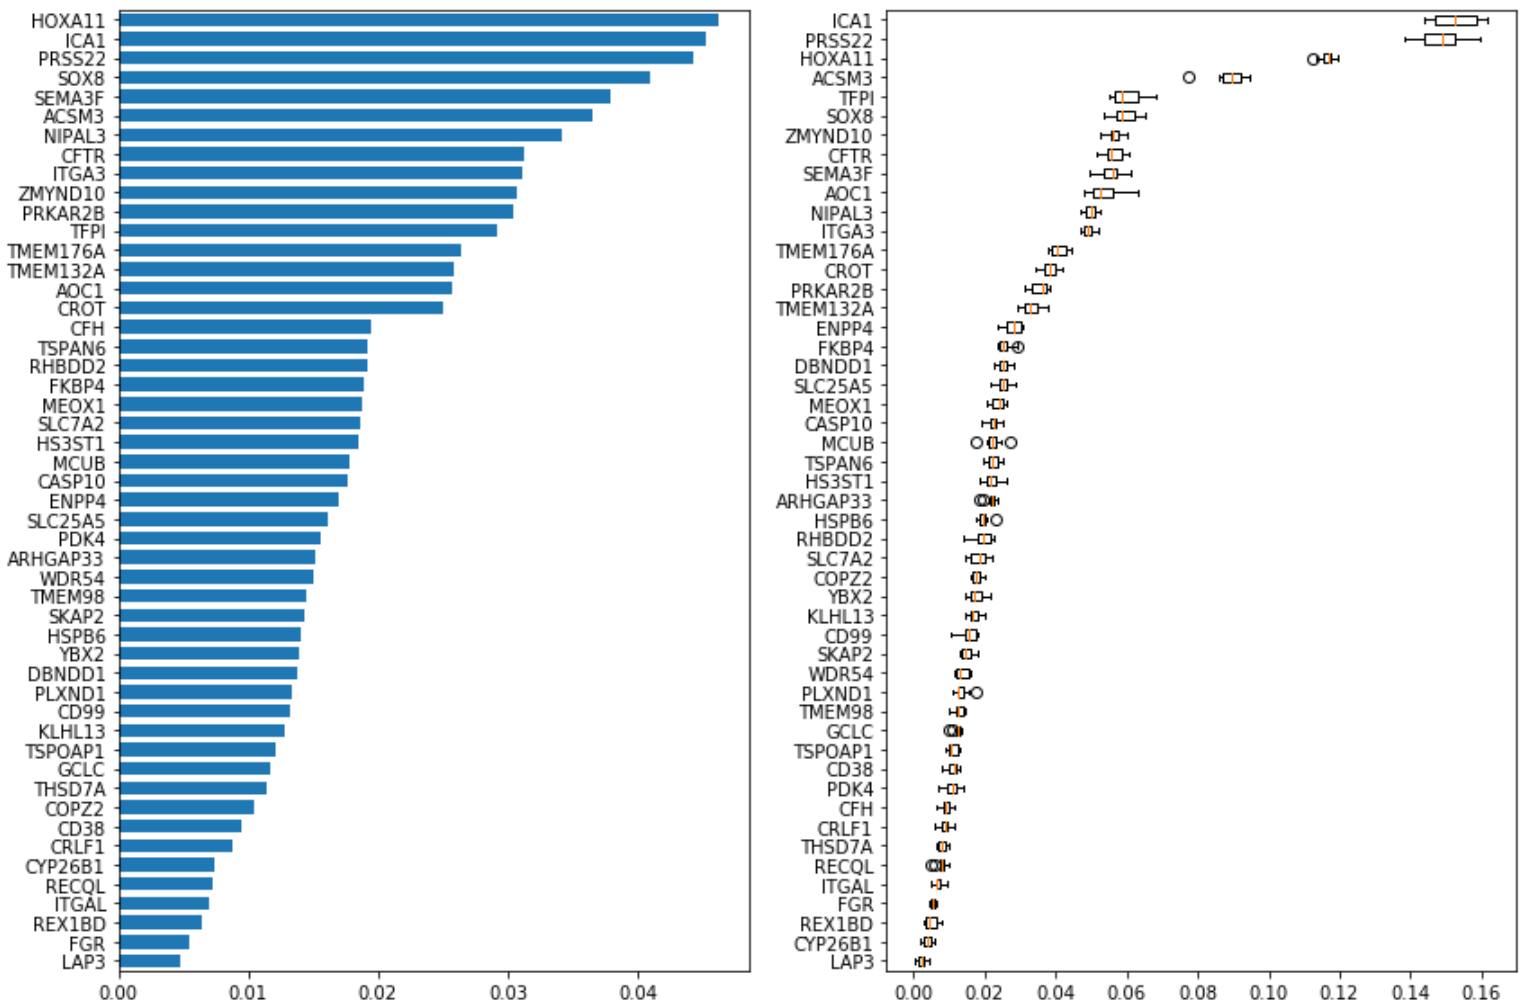
\includegraphics[scale=1.0]{images/rf_fi.png}
	\caption[Interpretation of marker genes]{Interpretation of marker genes per class with a gene effect score of minimum 0.25. Left: random forest-based permutation feature importance, right: $MCAE_{lrc}$ model-based feature importance. Genes and importance score are shown on y and x axis, respectively. }
    \label{fig:pfi}
\end{sidewaysfigure*}

\subsection{Finding common biomarkers}
Identifying all significant common genes will help understand various aspects for a specific cancer type~(e.g., BRCA carcinogenesis). Thus, these top genes have close relations to the corresponding tumor types, which could be viewed as potential biomarkers. \Cref{fig:comgenes} shows the top-10 common driver genes across 33 cancer types based on gene expression with Grad-CAM++ and LRP. 

\begin{figure*}[h]
	\centering
	\begin{subfigure}{.48\linewidth}
		\centering
		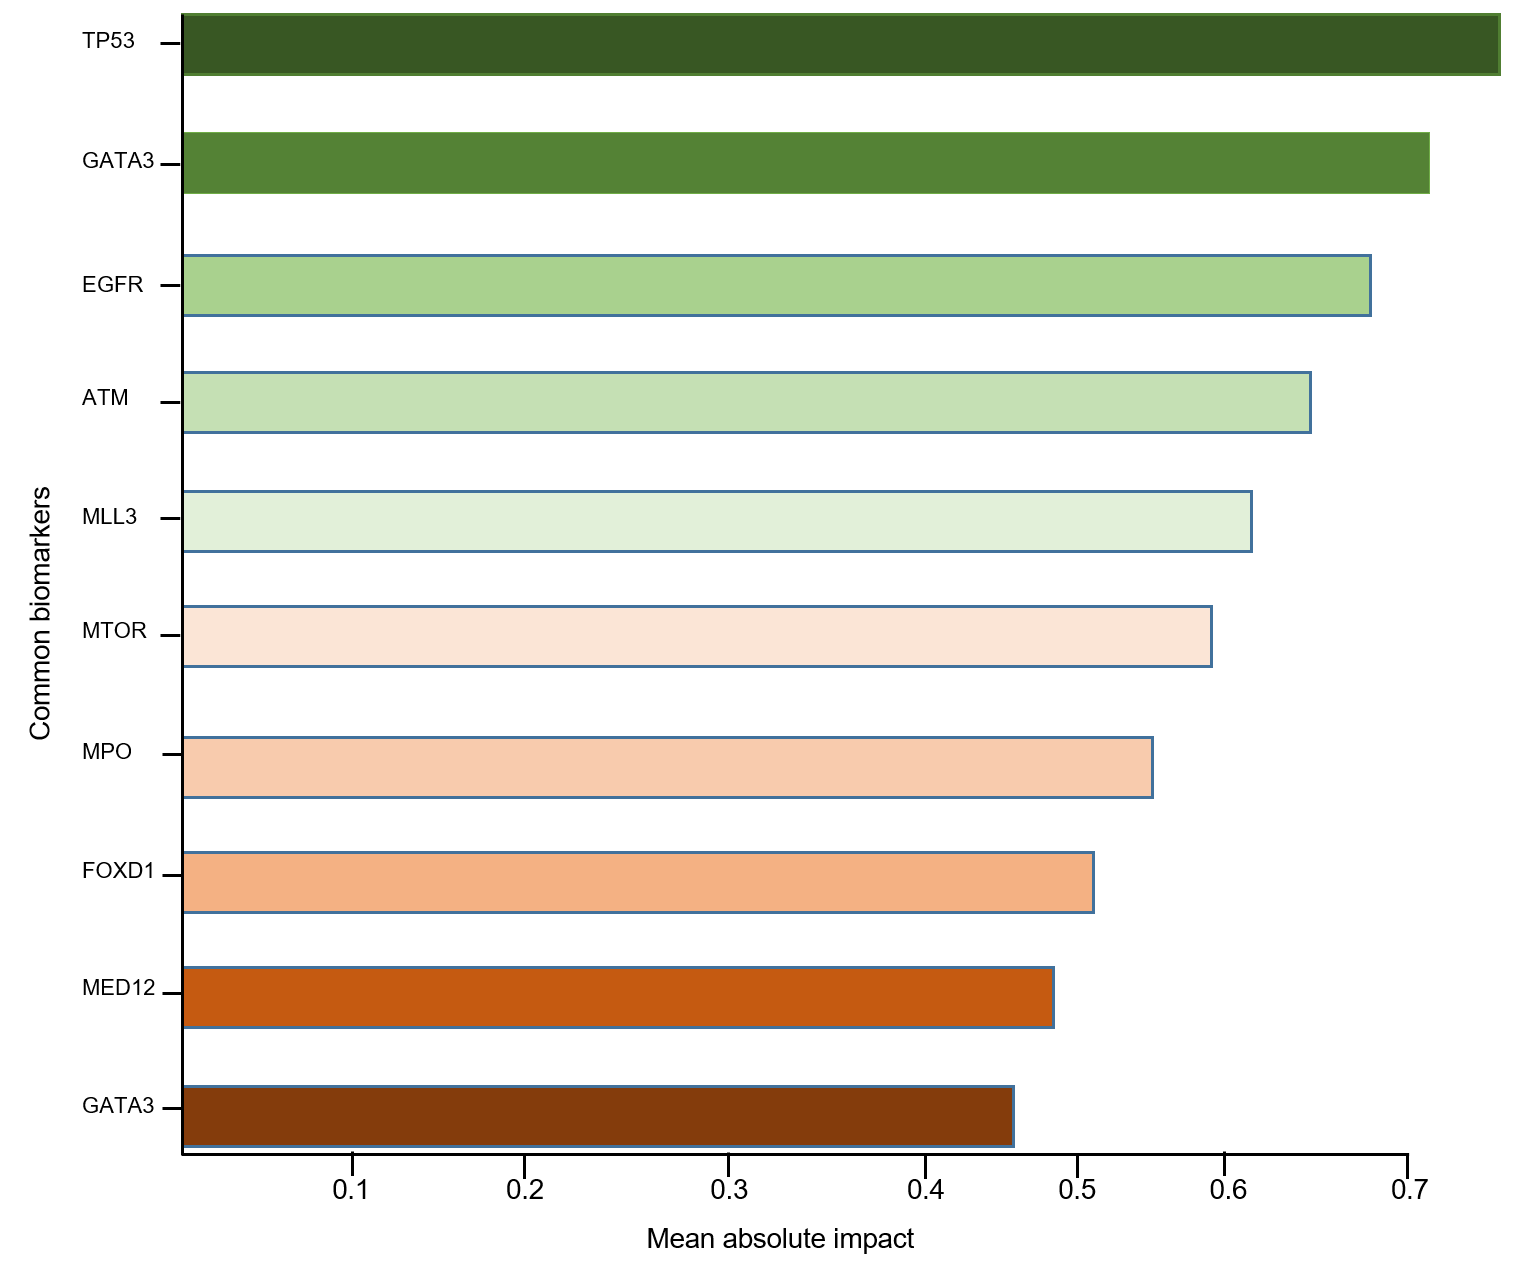
\includegraphics[scale=0.4]{images/gcam_fi.png}
		\caption{Grad-CAM++}
        \label{fig:comgenegcam}
	\end{subfigure}
	\begin{subfigure}{0.48\linewidth}
		\centering
		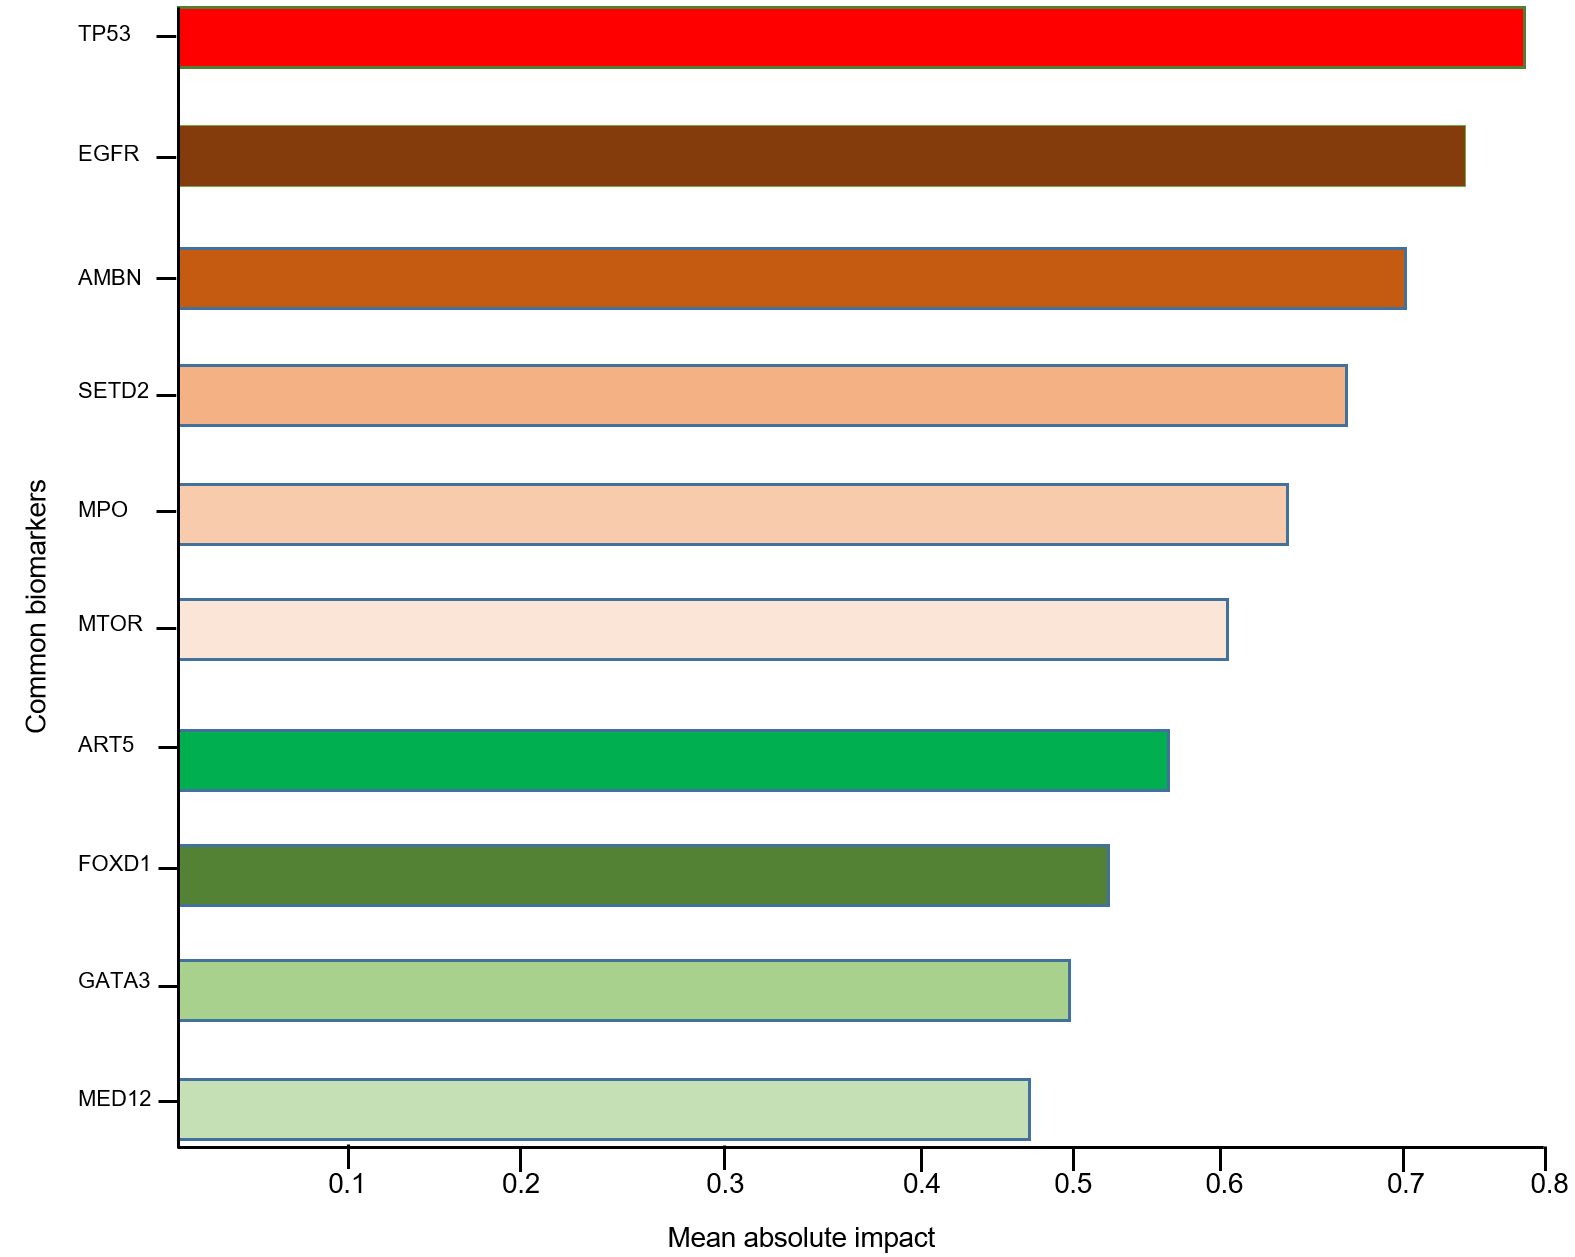
\includegraphics[scale=0.4]{images/lrp_fi.png}
		\caption{LRP}
        \label{fig:comgeneglrp}
	\end{subfigure}
	\caption{Common driver genes across 33 cancer types based on gene expression profiles} 
	\label{fig:comgenes}
\end{figure*}

\hspace*{3.5mm} As shown TP53, GATA3, EGFR, ATM, MLL3, MTOR, MPO, FOXD1, MED12, and GATA3 genes are identified as common driver genes across cancer types with Grad-CAM++, where TP53 protein-coding gene has the highest feature importance of 0.75. On the other hand, TP53, EGFR, AMBN, SETD2, MPO, MTOR, FOXD1, GATA3, and MED12 genes are identified as common driver genes across cancer types with Grad-CAM++, with the TP53 protein-coding gene having the highest feature importance of 0.78. 

\section{Chapter Summary}\label{chapter_5:conclusion}
In this chapter, we developed two deep multimodal architectures called $MCAE_{lrc}$ and $MCAE_{slr}$ cancer types based on different combination of multimodal genomics data types. Our approach is based on GradCAM++, LRP, and attention mechanism with a vanilla CNN, an VGG16, $MCAE_{lrc}$, and $MCAE_{slr}$ networks. Experiment results show that omics data are useful useful for predicting cancer types with high confidence giving high f1 scores~(of up to 96.25\% for single modality based on GE and of up to 92.45\% for GE+miRNA input modalities). Based on this comparison, we can conclude that there is a possibility both $MCAE_{lrc}$ and $MCAE_{slr}$ might surpass MAE and ML baselines models such as GBT or RF performance with the right combination of inputs. 
Our approach can predict cancer types 96.25\% of the cases correctly, which slightly outperforms the approach by Boyu et al.~\cite{lyu2018deep} but 6.5\% better than the approach by Yuanyuan et al.~\cite{li2017comprehensive}. 

\hspace*{3.5mm}Further, our approach reduces the false prediction rate for the READ, UCS, ESCA, and CHOL tumor samples. In particular, against 35\%, 81\%, 77\%, and 56\% of the correctly predicted cases by~\cite{lyu2018deep}, our approach predicts 88.74\%, 87.26\%, 89.56\%, and 84.55\%~(in cyan) cases correctly. Although slightly underperforms than~\cite{lyu2018deep} at classifying BRCA, THCA, and PRAD~(in red), our approach is more consistent for the majority cancer types and likely to perform more stably on new GE data. We also attempted to provide a more human-interpretable explanation by showing statistically significant biomarkers, which confirms that the identified genes are biologically relevant. 

\hspace*{3.5mm} However, several other factors have hindered this research, e.g., lack of enough training samples and single modality, i.e., only GE data used for making the predictions and generating the explanations. The latter reason caused the network to produce high training and validation errors during the training phase, giving lower accuracy during the inferencing phase. Although we attempted to open the CNN, VGG16, and MCAE `black-box' models through biomarker validation and feature ranking, our approach is mostly post-hoc as the explainability is based on test cases and results similar to LRP. 
Several further factors have hindered this research, such as lack of enough training samples, and lack of biological pathways analysis. On the other hand, In order to ensure an explainable model is robust to adversaries and behaves as intended in real-life treatment diagnosis, we need to use adversarial training to improve performance\cite{bhatt2020explainable}. In the next chapter, we will focus on improving the robustness of the multimodal interpretable model, particularly with a focus on adversarial robustness. 
